\chapter[Iterative Mapping of Probabilities: A data fusion framework for generating accurate land cover maps that match area statistics]{Iterative Mapping of Probabilities: A data fusion framework for generating accurate land cover maps that match area statistics}
\label{cha:chapter3}
\vspace*{\fill}
This chapter is based on:
\\
\\
% Full citation of the published (or submitted/in review) article
% This refers to the article key in the refs.bib file.
\fullcite{witjes2024iterative}
\newpage

\section*{Abstract}
% Core purpose
    Providing land cover estimates with both correct pixel-level class predictions and regional class area estimates is important for many monitoring and accounting purposes but rarely achieved by current land monitoring efforts. We propose a framework that uses class probabilities predicted by machine learning to guarantee that the mapped proportion of each class matches independent area estimates. 
    % Short methodology
    We used CatBoost models trained on CORINE data to predict probabilities for 8 primary LUCAS land cover classes in five European countries. We then used the proposed algorithm to produce proportional class maps that match Eurostat class area estimates. We validate these proportional class maps and baseline highest likelihood class maps with LUCAS land cover observations and S2GLC validation points.
    % Main findings
    Our results show that the framework and algorithms create maps that match area estimates, and that may also be more accurate than maps created with highest likelihood classification. This is especially the case with general-purpose models trained on data whose class proportions are not representative of the mapped area, which means that this algorithm can be used to localize such models for more accurate mapping of individual countries.

\newpage

\section{Introduction}
    % Why do we need area estimates and maps
    Land cover changes are fundamental to understanding the complex interplay between human activities and the environment \citep{winkler2021global}. Locating and quantifying this process is essential for several UN Sustainable Development Goals (SDG) \citep{unstats2023sdgs,romijn2016monitoring}, predicting and combating climate change \citep{unfccc2015adoption}, and preserving the diversity of life on earth \citep{cbd2016indicators}. For this, we currently rely on two main techniques: model-based mapping (pixel- or polygon based predictions) and design-based area estimation for a given region.
    
    % Area estimation from maps & its limitations
    Land cover maps enable visualization and analysis of spatial patterns, allowing the identification of drivers of change \citep{sy2019tropical}, quantifying carbon emissions \citep{avitabile2016carbon}, and targeted land management \citep{verburg2011challenges}. Design-based land area estimates, on the other hand, provide statistically-robust, model-free insights and estimates (typically with confidence intervals) of long-term trends and comparisons necessary for resource allocation, economic assessments, and international accountability \citep{olofsson2014good,gallego2017copernicus}. 
    As a result, policy and decision-makers often continue to rely on design-based area estimates, while there also is interest in maps that match the statistical area estimates. Due to the costs involved in performing such sampling surveys, there has long been a large interest in deriving area estimates directly from Earth Observation \citep{gallego2004remote}. Counting the number of pixels per class in the mapped area is the simplest method, but strongly discouraged due to unpredictable biases that may lead to over- and under-prediction of specific classes \citep{gallego2004remote,olofsson2014good,waldner2017where}. These area biases stem from many sources such as imbalanced training data \citep{he2009learning,mellor2015exploring,zhu2016optimizing}, the interaction between spatial resolution and pixel heterogeneity \citep{strahler2006global,herold2008challenges}, regional accuracy differences \citep{waldner2016towards,witjes2022spatiotemporal,duarte2023thematic}, and classifier design \citep{waldner2016towards,ghorbani2020comparing,demirkaya2020exploring}, and are therefore difficult to quantify in order to assess the uncertainty of predictions. 
    
    % Supplementing area estimates with mapping
    Unbiased area estimation based on pixel counting is possible using the confusion matrix computed from additional statistical reference data that are e.g. stratified according to the mapped classes. The map-based area estimates are then adjusted using commission and omission errors from according to the confusion matrix \citep{stehman2013estimating,stehman2014estimating,olofsson2013making,olofsson2014good}. 
    While it is not always feasible to obtain additional samples directly from the mapped area, many organizations still adhere to this approach as their standard practice. This is primarily because methods that rely on obtaining (additional) samples directly from the field tend to yield more precise area estimates compared to other methods \citep{finegold2016map,gallego2017copernicus,redd2022estimating,angelopoulos2023predictionpowered}.
    Recent developments suggest that unbiased area estimation may be possible without requiring post-classification sampling. For instance \citep{kleinewillinghofer2022unbiased} used Land Use/Cover Area Frame Survey (LUCAS) data and Copernicus High Resolution Layers (HRL) layers to show that it may be possible when the sampling design of the reference data is appropriate for the mapped phenomenon. Furthermore, \citet{sales2022land} derived area estimates from probabilities predicted by a random forest that were  more accurate than pixel counting in a binary classification context. Finally, the prediction-powered inference framework recently proposed by \citet{angelopoulos2023predictionpowered} makes it possible to derive quantity estimates with statistically valid confidence intervals that are smaller than those of purely sample-based estimates, without the need for post-classification sampling to adjust for model bias.
    
    % Use existing area estimates
    While these approaches show promise towards the end goal of deriving unbiased and accurate area estimates without requiring additional sampling, policy and decision makers continue to rely on sample-based area estimates such as the European Commission's LUCAS \citep{gallego2017copernicus}, and require maps that match their class proportions to enable localized interventions \citep{olofsson2014good}. Linking trends from area estimates to periodic maps would also facilitate temporally and spatially explicit assessment of land change, which is crucial for evaluating the impacts of critical human activities on the environment \citep{olofsson2014good,szantoi2020addressing,winkler2021global}. A key issue is that land cover monitoring from remote sensing data has been producing accurate spatial maps or providing "best" area estimates but rarely the focus has been on addressing both objectives together: an accurate map whose spatial distribution of classes is an exact match to those from a provided, trusted area estimate. This would effectively minimize both allocation and quantity disagreement \citep{pontius2011death}; pixel-wise classification errors and map-wide class quantities, respectively. Although this issue has been subject to study since the early years of remote sensing \citep{strahler1980use}, little research on related approaches has been presented so far. \citet{janssen1992knowledge} showed that using ancillary data about class area proportions can be used to improve classification accuracy, especially when there is uncertainty caused by 'mixed pixels' or difficulty separating classes in the feature space. \citet{mingguo2009effect} further analyzed such methods and showed that using prior probabilities to adjust classification thresholds can be used to change the balance of user's and producers's accuracy (precision and recall, respectively), but that this can cause small classes to disappear from the classified map. There have been few attempts to use ancillary data to go beyond improving per-pixel accuracy and actually making maps that match area estimates. A notable exception is the work done by \citet{troltzsch2009spatial} and \citet{brus2012statistical}, who made 1~km within-pixel tree species proportion maps of Europe, and used an iterative scaling and calibration technique to make them correspond to national forest statistics. 
    
    % Horvaths method
    More recently, \citet{horvath2021comparison} transformed predicted probability surfaces for vegetation types \citep{horvath2019distribution} into classified maps whose class distributions matched estimates derived from area frame survey data \citep{bryn2018land}, iterating over each species and assigning pixels on the map to that species until the expected prevalence was reached. However, they found that while their proposed methods produced maps with correct area proportions, these maps were less accurate than a map where each pixel was assigned to the class with the highest predicted probability, which suggests a trade-off between allocation and quantity disagreement. Furthermore, their proposed method left approximately 10\% of the map unclassified because not every pixel had probabilities for every class. 
    As soon as a pixel is assigned to one class, it can no longer be assigned to another; if pixels with probabilities above 0 for a certain class are rare, this leaves gaps in the classified map that must be filled with other methods.     
    We hypothesize that the amount of remaining unclassified pixels can be reduced by using 'smoother' input probability data. We consider such data 'smooth' when for each class, there are more pixels with a predicted probability value above zero than the number of required pixels on the final map. 
    This might be achieved by improving a model's ability to generalize such as using a bigger training dataset. This is often unfeasible in land cover classification due to the cost involved in collecting reference data, especially when area proportions must be correctly represented to obtain matching proportional predictions \citep{sales2022land,kleinewillinghofer2022unbiased}. \citet{horvath2021comparison} state that the accuracy of their proportional maps might be improved by using more accurately predicted input probabilities, and models trained on bigger training datasets tend to be more accurate \citep{myburgh2014impact,rodriguez-perez2017influence}. While there are general recommendations for training dataset size \citep{foody2006training,koshute2021recommending} and indications that tree-based methods can attain high accuracy without large training datasets \citep{ramezan2021effects} it is important to represent as much of the feature space as possible \citep{meyer2021predicting,wadoux2019sampling}. Furthermore, \citet{witjes2022spatiotemporal,witjes2023ecodatacube} showed that models trained on larger portions of CORINE-derived training data generalized better on unseen data, especially when mapping land cover in years not covered by the training dataset.
    
    % What are we doing in this paper
    This paper proposes and demonstrates a framework that employs predicted probabilities for land cover classes to create land cover maps that are both accurate and adhere to the class distribution determined by independent area estimates. We present an expanded version of the approach suggested by \citet{horvath2021comparison} that iterates over each class multiple times to minimize the overlap between classes: Iterative Mapping of Probabilities (IMP). We investigate the effectiveness and potential advantages of the proposed approach by answering the following research questions:
        
    \begin{enumerate}
    \item How does the quantity disagreement vary between proportional maps produced by IMP compare to that of highest likelihood class maps?
    \item How does the allocation disagreement vary between proportional maps and highest likelihood class maps?
    \item What is the impact of using machine learning models trained on national or larger area training datasets for producing proportional maps?
    \end{enumerate}

    We will answer these questions by creating proportional and highest likelihood class maps for five European countries. We will measure quantity disagreement by comparing the proportion of predicted classes to EuroStat area estimates, and allocation disagreement by validating the maps LUCAS land cover samples and S2GLC validation points. To assess the impact of using larger but less proportional training datasets, we do this twice: Once with a model trained on land cover data from the mapped country, and once with a model trained on a data from a group of countries.
        
\section{Materials and Methods}

    In this study, we classify land cover and produce maps that match area estimates by Eurostat across five neighboring European countries: Belgium, Czechia, Germany, Luxembourg, and The Netherlands. We utilized CORINE training points produced by \citep{witjes2022spatiotemporal}, from which we removed potential labeling errors using data from Copernicus HRL and OpenStreetMap. CatBoost classification models were then trained on these filtered points, with distinct models trained on subsets of the CORINE points from each country (referred to as \emph{local models}) and one \emph{general model} trained on CORINE points from all countries that adopted the LUCAS survey in 2006: Belgium, Czechia, France, Germany, Hungary, Italy, Luxembourg, The Netherlands, Poland, and Slovakia. For each of the five mapped countries, we predicted LUCAS land cover probabilities with the country's local model, as well as with the general model for the years 2009, 2012, 2015, 2017, and 2018. Each set of probabilities was used to create two hard-class land cover maps: One \emph{highest likelihood class map} created through highest likelihood classification, and one \emph{proportional class map}, created by the proposed algorithm in an attempt to match land cover class quantities with official LUCAS estimates. We validated our annual maps of 2009, 2012, 2015 and 2018 with the LUCAS points compiled by \citep{dandrimont2020harmonised}. The maps for 2017 were validated with a separate dataset that was explicitly created to validate the S2GLC land cover map of 2017 \citep{jenerowicz2021validation}. We used this evaluation to compare the classification performance of local and  general models, as well as highest likelihood class maps and proportional maps. An overview of our methodology is provided in Fig.~\ref{fig:workflow}.

    \begin{figure}
    \centering
    \includegraphics[width=\linewidth]{figs_04/fig1_methodology.pdf}
    % https://drive.google.com/file/d/1jB1FImQ1uke8RK1EKRSCaRF7iKUca4VG/view?usp=sharing
    \caption{Overview of the methodology to produce, validate, and compare highest likelihood and proportional maps. More detailed information on the production of the training data and features can be found in \citep{witjes2022spatiotemporal} and \citep{witjes2023ecodatacube}.}
    \label{fig:workflow}
    \end{figure}
    
    \subsection{Training and reference data}
    
        We used three different land cover point datasets for this study: 1) centroids of CORINE land cover polygons from 2006, 2012 and 2018 extracted by \citet{witjes2022spatiotemporal} (available on Zenodo \citep{landa2021multi}), 2) in-situ LUCAS samples of harmonized by \citet{dandrimont2020harmonised}, and 3) validation points of S2GLC land cover maps \citep{malinowski2020automated} produced by \citet{jenerowicz2021validation} (see Fig.~\ref{fig:points}). All classifiers were trained using CORINE centroids as reference, and all produced maps were validated on S2GLC and LUCAS samples. The strict sampling design and high accuracy of the LUCAS survey has made it a valuable resource in training and validating land cover models across Europe \citep{benevides2021land,pflugmacher2019mapping,sparks2022mapping,verhegghen2021accuracy,witjes2022spatiotemporal}, while S2GLC was specifically designed to validate land cover maps of Europe, using a stratified random sampling design to ensure proportional coverage of all European countries equal or larger in size than Luxembourg (see section 2.4 of \citet{malinowski2020automated}).

        \begin{figure}
        \centering
        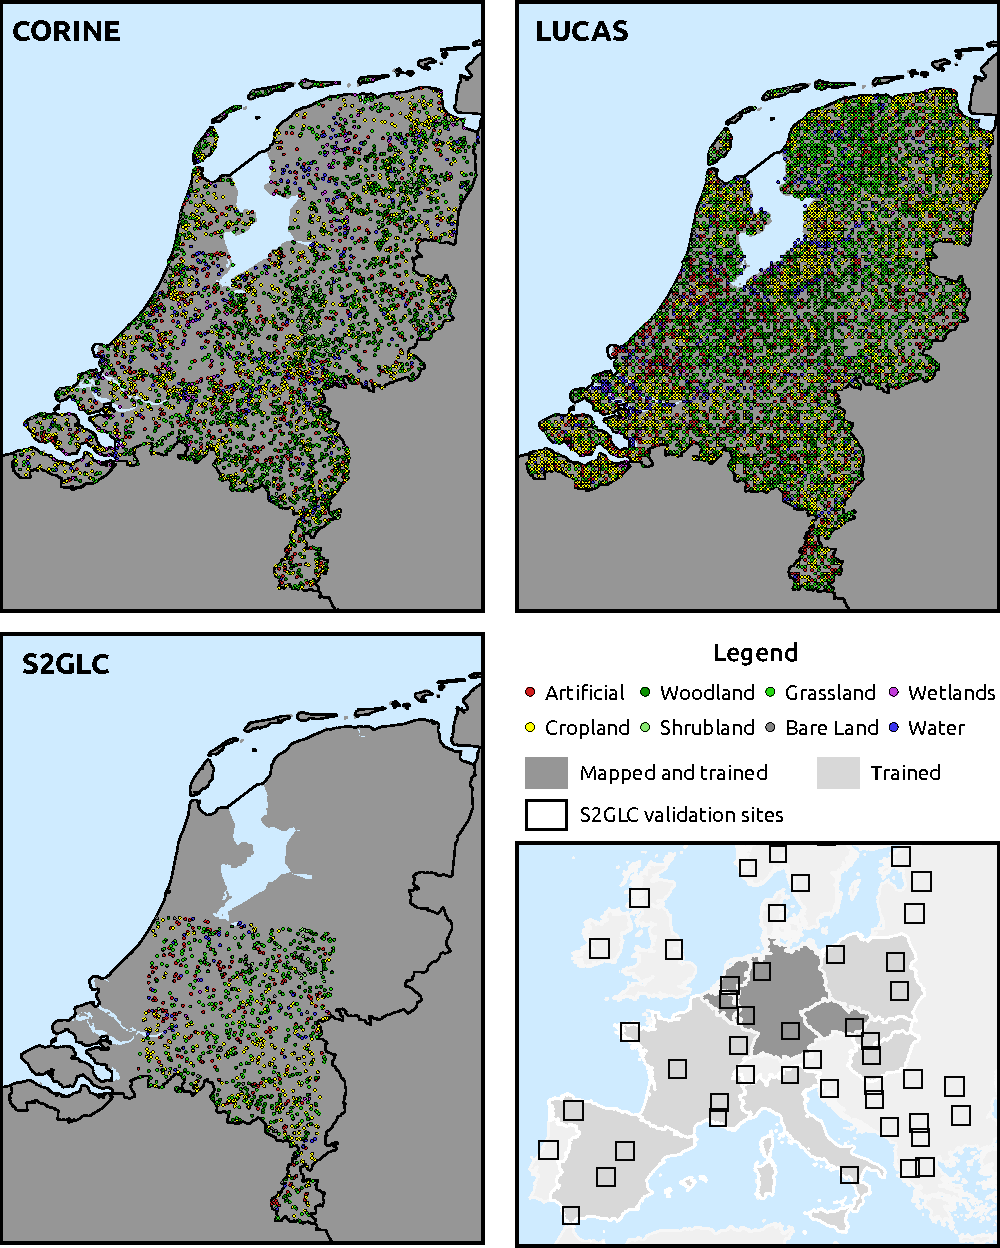
\includegraphics[width=0.9\linewidth]{figs_04/fig2_points.pdf}
        
        \caption{Example of the distribution of CORINE training data \citep{witjes2022spatiotemporal}, LUCAS validation data \citep{dandrimont2020harmonised}, and S2GLC validation data \citep{jenerowicz2021validation}, each subset to the Netherlands to visualise their spatial distribution. Bottom right: An overview of countries and S2GLC validation sites surrounding the area of interest. Countries that were mapped and from which CORINE training data was extracted ("\textit{Mapped and trained}") are marked in dark gray, while countries from which additional CORINE points were extracted for the general model (\textit{"Trained"})are marked in light gray.}
        \label{fig:points}
        \end{figure}

    \subsubsection{Legend harmonization and filtering}
    
        We reclassified all CORINE-derived and S2GLC points to eight LUCAS land cover classes (level-1). In the case of CORINE points, we removed any points that belong to CORINE classes with no clear and exclusive match to a LUCAS class. This process was conducted according to the key shown in table \ref{tab:clc3_to_lucas1}

        Considering that the minimum mapping unit of CORINE is 25 hectares and the minimal width of mapped features 100m, CORINE polygons can encompass smaller-scale land cover types that differ from the main category of the polygon, introducing a risk of labeling errors. We counteracted this by screening the CORINE-derived points and removing all points whose land cover class were inconsistent with data from Copernicus HRL layers and OpenStreetMap in a similar way as the one detailed in \citet{witjes2022spatiotemporal}. For example, grassland training points were removed if Copernicus HRL layers indicated tree cover, or if OpenStreetMap rasters indicated roads or buildings were present at the points' coordinates. \ref{tab:corine_filtering} provides an overview of the data and conditions used to remove potentially faulty training points for each class.
    
        \begin{table}[H]
        \centering
        \caption{Reclassification key of CORINE and S2GLC land cover codes to LUCAS level 1 land cover. CORINE centroids of classes in the \textit{Not Used} category were removed from the training set.}
        \label{tab:clc3_to_lucas1}
        \begin{tabular}{lll}
        \hline
        LUCAS land cover & CORINE codes                             & S2GLC codes  \\ 
        \hline
        Artificial       & 111, 112, 121, 122, 132, 133             & 111          \\
        Cropland         & 211, 212, 213, 221, 222, 223, 241        & 211, 221     \\
        Woodland         & 311, 312, 313                            & 311, 312     \\
        Shrubland        & 322, 323, 324                            & 322          \\
        Grassland        & 231, 321                                 & 231          \\
        Bare land        & 331, 332, 333, 334, 335                  & 331, 335     \\
        Wetlands         & 411, 412, 421, 422, 423                  & 411, 412     \\
        Water            & 511, 512, 521, 522, 523                  & 511          \\ 
        \hline
        Not used         & 123, 124, 131, 141, 142, 242, 243, 244   &          \\
        \hline
        \end{tabular}
        \end{table} 


    \subsubsection{Feature space}
        All training points were overlaid on 224 covariates: Landsat data, derived spectral indices, a digital terrain model, and monthly minimum and maximum geometric temperature. 
        
        The Landsat data were originally published by \citet{potapov2020landsat}, aggregated to seasonal composites and gap-filled with a temporal moving window median (TMWM) algorithm by \citet{witjes2023ecodatacube}, and are openly available for download on \url{stac.ecodatacube.eu}. From the original bands (Blue, Green, Red, NIR, SWIR1, SWIR2, Thermal), several spectral indices were calculated: 
        \begin{enumerate}
            \item Normalized Difference Vegetation Index (NDVI) \citep{rouse1974monitoring}, 
            \item Soil Adjusted Vegetation Index (SAVI) \citep{huete1988soil}, 
            \item Modified Soil Adjusted Vegetation Index (MSAVI) \citep{qi1994modified}, 
            \item Normalized Difference Water Index (NDWI)  \citep{mcfeeters1996use}
            \item Normalized Difference Moisture Index(NDMI) \citep{gao1996ndwi},
            \item Normalized Burn Ratio (NBR) \citep{garcia1991mapping}, 
            \item Normalized Burn Ratio Plus (NBR+) \citep{alcaras2022normalized},
            \item Road Extraction Index (REI) \citep{shahi2015novel}, 
            \item Enhanced Vegetation Index (EVI) \citep{liu1995feedback}
        \end{enumerate}
        For each Landsat band and spectral index, the highest 25th percentile, median, and 75th percentile was included for each of the 4 seasons typical in Central Europe, resulting in 12 covariates for each of 7 bands and 8 indices, amounting to 192 Landsat-derived covariates.

        The digital terrain model was originally published by \citet{hengl2020continental}. We used 8 derived variables:
        \begin{enumerate}
            \item Slope percent
            \item Elevation (Lowest mode)
            \item Northness
            \item Easterness
            \item Positive openness \citep{yokoyama2002visualizing}
            \item Negative openness \citep{yokoyama2002visualizing}
            \item Multidirectional hillshade \citep{mark1992multidirectional}
            \item 315 degree sun azimuth hillshade \citep{mark1992multidirectional}
        \end{enumerate}
        
        The minimum and maximum geometric temperature is a geometric transformation of latitude and the day of the year \citep{kilibarda2014spatio}. Aggregated to monthly averages, this amounts to 24 covariates.

    \subsubsection{Area estimates}

        The area estimates used as input for the proposed algorithm, and to validate the quantity disagreement of all produced maps, were obtained from Eurostat \citep{eurostat_lucas}. This database reports how much of each LUCAS land cover class covers each country in each year that the LUCAS survey was performed: 2006, 2009, 2012, 2015, and 2018. We derived proxy area estimates for 2017 through linear interpolation of the area estimates of 2015 and 2018.
    
    \subsection{Machine learning}
    
        We trained CatBoost classifiers on the filtered and overlaid CORINE-derived points. CatBoost is an implementation of gradient boosting \citep{prokhorenkova2018catboost} that has seen much use in recent years due to its ability to achieve relatively high accuracy on large datasets in several fields \citep{hancock2020catboost}, notably being used to produce ESA WorldCover \citep{zanaga2022esa} and WorldCereal \citep{tricht2023worldcereal}. 
        
        %old= To study whether a larger feature space compensates for a class distribution that less closely matches the distributions of the target area, we created separate models trained only on samples from each country, as well as one model trained on samples from all countries that participated in the LUCAS program in 2006, resulting in five \textit{local} models and one \textit{general} model (see table \ref{tab:total_samples}).

        We trained six models in total: five \textit{local} models trained exclusively on CORINE training data from each country, and one \textit{general} model trained not only on data from the five countries, but also on CORINE data from all countries that participated in the LUCAS program in 2006. Each model was trained on CORINE data from all available years: 2006, 2012, and 2018. Table \ref{tab:total_samples} shows how many training points were used for the local models of each country, with the column \textit{Other} representing the countries from which training data was extracted, but which were not mapped by a local model (see also Fig. \ref{fig:points}). We included this general model in our analysis to investigate whether a larger feature space compensates for a less balanced class distribution.
        
        \begin{table}[H]
        \caption{Summary of CORINE points per country and LUCAS level 1 class, used to train the land cover models in this work. Local models were only trained on the available points for that country, while the general model was trained on all points, including those from other countries.}
        \label{tab:total_samples}
        \resizebox{\linewidth}{!}{%
        \begin{tabular}{lrrrrrrr}
        Lucas class & Belgium & Czechia & Germany & Luxembourg & Netherlands & Other   & Total \\
        \hline
        Woodland    & 13,661   & 46,555   & 202,657  & 1,575      & 4,934        & 683,623  & 953,005  \\
        Cropland    & 12,637   & 25,506   & 112,383  & 1,104      & 3,608        & 512,865  & 668,103  \\
        Grassland   & 10,176   & 21,923   & 69,541   & 689       & 2,647        & 255,673  & 354,649  \\
        Artificial  & 2,028    & 3,286    & 19,274   & 170       & 2,046        & 65,012   & 90,816   \\
        Shrubland   & 494     & 1,005    & 2,932    & 11        & 614         & 144,393  & 150,449  \\
        Water       & 451     & 1,994    & 8,415    & 20        & 1,222        & 25,085   & 37,187   \\
        Wetlands    & 50      & 272     & 2,903    & 3         & 584         & 8,385    & 12,197   \\
        Bare land   & 41      & 18      & 833     & 0         & 152         & 31,431   & 32,475   \\
        \hline
        Total       & 39,538   & 100,559  & 418,938  & 3,572      & 15,807       & 1,726,467 & 2,250,881 \\
        \hline
        \end{tabular}}
        \end{table}
    
        The training points were split up into 2996 30~km tiles. We randomly selected 5\% of these tiles as validation data. The remaining points were used to train all models. To prevent overfitting, we validated each model after each iteration on the points from the validation tiles. Training was automatically stopped when validation accuracy had not improved for 10 consecutive epochs, and the model resulting from the epoch where the most recent validation accuracy improvement was recorded was selected as the final model.
    
    \subsection{Land Cover Classification}
        For each country, we predicted probabilities for the eight LUCAS land cover classes in the years 2009, 2012, 2015, 2017 and 2018. We did this once with that country's local model, and once with general model. For each set of predicted probabilities, we created a \textit{highest probability class map} (HPC) by assigning each pixel to the class having the highest class probability. This resulted in ten highest probability class maps per country (five years,times two models).


    \subsection{Iterative Mapping of Probabilities}
    We implemented IMP, a post-processing algorithm, on each set of predicted probabilities (year, country, model). IMP is designed to create the most accurate possible hard-class map with 1) a given set of predicted probabilities and 2) an existing area estimate, based on the following assumptions: 
    \begin{enumerate}
        \item \textbf{Bias between classes} Models can have unknown biases and may overpredict certain classes by assigning relatively higher probabilities for them on average, which leads to rarer classes being underrepresented by highest likelihood classification \citep{he2009learning,waldner2017where}.
        \item \textbf{Ranking within classes} Within each class, the pixels with higher predicted values are more likely to correspond with actual occurrence of that class in a given pixel, regardless of the predicted probability values for other classes in the same pixel. Essentially, even if all probabilities for a single class are relatively low, they are at least roughly ranked in the correct order of likelihood for a given class. This is not always guaranteed \citep{niculescu2005predicting}, but can generally can be expected from accurate classifiers.
        \item \textbf{Overlap between classes:} When selecting pixels based on the level of their within-class relative probability, some pixels may be the best candidates for multiple classes (i.e. being in the top percentile of probabilities), either due to model bias, or due to multiple classes actually occurring inside the same pixel \citep{horvath2021comparison}.
    \end{enumerate}

    In general, IMP functions similar to the method proposed by \citet{horvath2021comparison}: It loops over every class, selecting the pixels with the highest predicted probability for that class and assigns the corresponding pixels on the output map to that class. However, to minimize the overlap problem, IMP does not do this once, but several times, each time selecting only the top percentile of available pixels for each class. We set the number of iterations to 20 in our presented experiments. This means that at every iteration, IMP selects the best 5\% of the target proportion from the best available pixels for each class.
    For example, a class which was estimated to cover 20\% of a country's surface, at the first iteration, only the pixels with 0.2\% of that class' highest predicted probabilities will be assigned to that class. At the second iteration, it would select and the pixels that are within 0.4\% of that range, but some of those pixels will have been assigned to other classes. Instead, it will select the pixels with the top 0.2\% highest probabilities for that class \textit{amongst the remaining unassigned pixels in the output map}. Figure~\ref{fig:imp} presents a visualisation of how IMP gradually fills a map until the proportions of each class matches those in the target area estimate. A detailed description of IMP is provided in \ref{alg:imp}.

    \begin{figure}[H]
        \centering
        % https://app.diagrams.net/#G1jB1FImQ1uke8RK1EKRSCaRF7iKUca4VG#%7B%22pageId%22%3A%22ZHYfUoFFE5HdqB9tgYix%22%7D
        \includegraphics[width=0.9\textwidth]{figs_04/fig3_imp.pdf}
        \caption{Visualisation of how IMP gradually classifies each pixel in the study area, selecting the pixels with the highest available probabilities for each class in each iteration.}
        \label{fig:imp}
    \end{figure}

    \subsection{Accuracy Assessment}
    
    We assess the allocation and quantity disagreement \citep{pontius2011death} of the produced models and maps by validating the maps of 2009, 2012, 2015 and 2018 with LUCAS points \citep{dandrimont2020harmonised} and the maps of 2017 with S2GLC points \citep{jenerowicz2021validation}. Table~\ref{tab:total_lucas} shows the support per class per country for LUCAS points, and table~\ref{tab:total_s2glc} for the S2GLC points. We quantify allocation disagreement with the Weighted F1-score metric \citep{rijsbergen1980information}, a harmonic mean of user's and producer's accuracy (precision and recall), because it distinguishes classification performance more strictly on datasets with imbalanced class distributions. This makes it a useful metric to compare the classification performance when both accuracy and proportion of each class are important. This is done both for the \textit{highest likelihood} class maps (based on the highest probability per point or pixel) and the \textit{proportional} class maps produced by IMP. We measure quantity disagreement with the percentage that class-wise proportions of each map deviate from the area assessment of the target country in the target year.

    \begin{table}[H]
        \caption{Summary of LUCAS points per country and LUCAS level 1 class, used to validate the land cover maps of 2009, 2012, 2015, and 2018}
        \label{tab:total_lucas}
        \resizebox{\linewidth}{!}{%
        \begin{tabular}{lllllll}
        \toprule
        Lucas class & Belgium & Czechia & Germany & Luxembourg & Netherlands &   Total \\
        \midrule
         Artificial &   1,365 &   1,120 &   8,911 &         83 &       1,742 &  13,221 \\
           Cropland &   4,006 &  10,487 &  47,926 &        285 &       4,147 &  66,851 \\
           Woodland &   2,902 &   8,552 &  34,813 &        347 &       1,845 &  48,459 \\
          Shrubland &     139 &     218 &   1,042 &         15 &         271 &   1,685 \\
          Grassland &   4,332 &   6,199 &  30,540 &        402 &       6,014 &  47,487 \\
          Bare land &     236 &     306 &   1,332 &         13 &         286 &   2,173 \\
           Wetlands &     150 &     283 &   1,786 &          8 &         720 &   2,947 \\
              Water &      42 &      62 &     542 &          0 &         101 &     747 \\
              Total &  13,172 &  27,227 & 126,892 &      1,153 &      15,126 & 183,570 \\
        \bottomrule
        \end{tabular}}
    \end{table}

    \begin{table}[H]
        \caption{Summary of S2GLC points per country and LUCAS level 1 class, used to validate the land cover maps of 2017}
        \label{tab:total_s2glc}
        \resizebox{\linewidth}{!}{%
        \begin{tabular}{lrrrrrr}
        \toprule
        Lucas class & Belgium & Czechia & Germany & Luxembourg & Netherlands & Total \\
        \midrule
         Artificial &     115 &      39 &     183 &          8 &         193 &   538 \\
           Cropland &     325 &     439 &   1,211 &         16 &         246 & 2,237 \\
           Woodland &     225 &     258 &   1,039 &         23 &         202 & 1,747 \\
          Shrubland &       2 &       1 &       8 &          0 &          18 &    29 \\
          Grassland &     200 &      60 &     459 &         17 &         329 & 1,065 \\
          Bare land &      15 &      14 &      42 &          0 &          21 &    92 \\
           Wetlands &      12 &       6 &      10 &          0 &          49 &    77 \\
              Water &       2 &       0 &      23 &          0 &           7 &    32 \\
              Total &     896 &     817 &   2,975 &         64 &       1,065 & 5,817 \\
        \bottomrule
        \end{tabular}}
    \end{table}
    
\section{Results}

    \subsection{Training data preprocessing}

    The LUCAS/CORINE training dataset used by \citep{witjes2022spatiotemporal} contained 3,381,460 CORINE centroids with CORINE classes that were compatible to the LUCAS level 1 legend. Filtering the CORINE centroids with Copernicus HRL and OpenStreetMap data removed 1,076,579 points, or 31.84 percent of the data. \ref{tab:corine_filtering} presents a full overview of the amount of training points removed by each filtering rule. 

    \subsection{Land cover classification and Proportional Post-Processing}

    Predicting eight land cover classes for five years with two models (a country-specific local model and a common general model) resulted in 80 predicted probability layers per country. Creating hard-class maps with highest likelihood classification yielded one map with eight classes for each year and each country, resulting in 25 hard-class maps. 
    
    Applying the algorithm in 20 iterations on the probabilities predicted by a country-specific local model and the general model produced an equal number of proportional class maps each country, year, and model type. Fig.~\ref{fig:big_map_proportional} shows the proportional land cover map of the entire study area for 2009, based on probabilities predicted by the LUCAS mode. Fig.~\ref{fig:map_example} shows an example of the iterative classification process resulting in a proportional land cover map, as well as a comparison with the highest likelihood map and the iteration at which each pixel was filled. Note that pixels that were classified at later iterations tend to also be marked as differences with the highest likelihood map, and that there are distinct spatial patterns in their occurrence: For instance, the edges of the grassland patches in the northern part of the area, the suburban part in the southern area, and the urban green areas in the city proper.

    \begin{figure}[H]
        \centering
        \includegraphics[width=\linewidth]{figs_04/fig4_map.pdf}
        \caption{LUCAS Land cover maps of Belgium, Czechia, Germany, Luxembourg and the Netherlands of 2009 generated with the proposed algorithm, using Eurostat national area estimates and probabilities predicted by the general CatBoost model trained on CORINE centroid points from all countries that implemented LUCAS in 2006.}
        \label{fig:big_map_proportional}
    \end{figure}
    
    \begin{figure}[H]
        \centering
        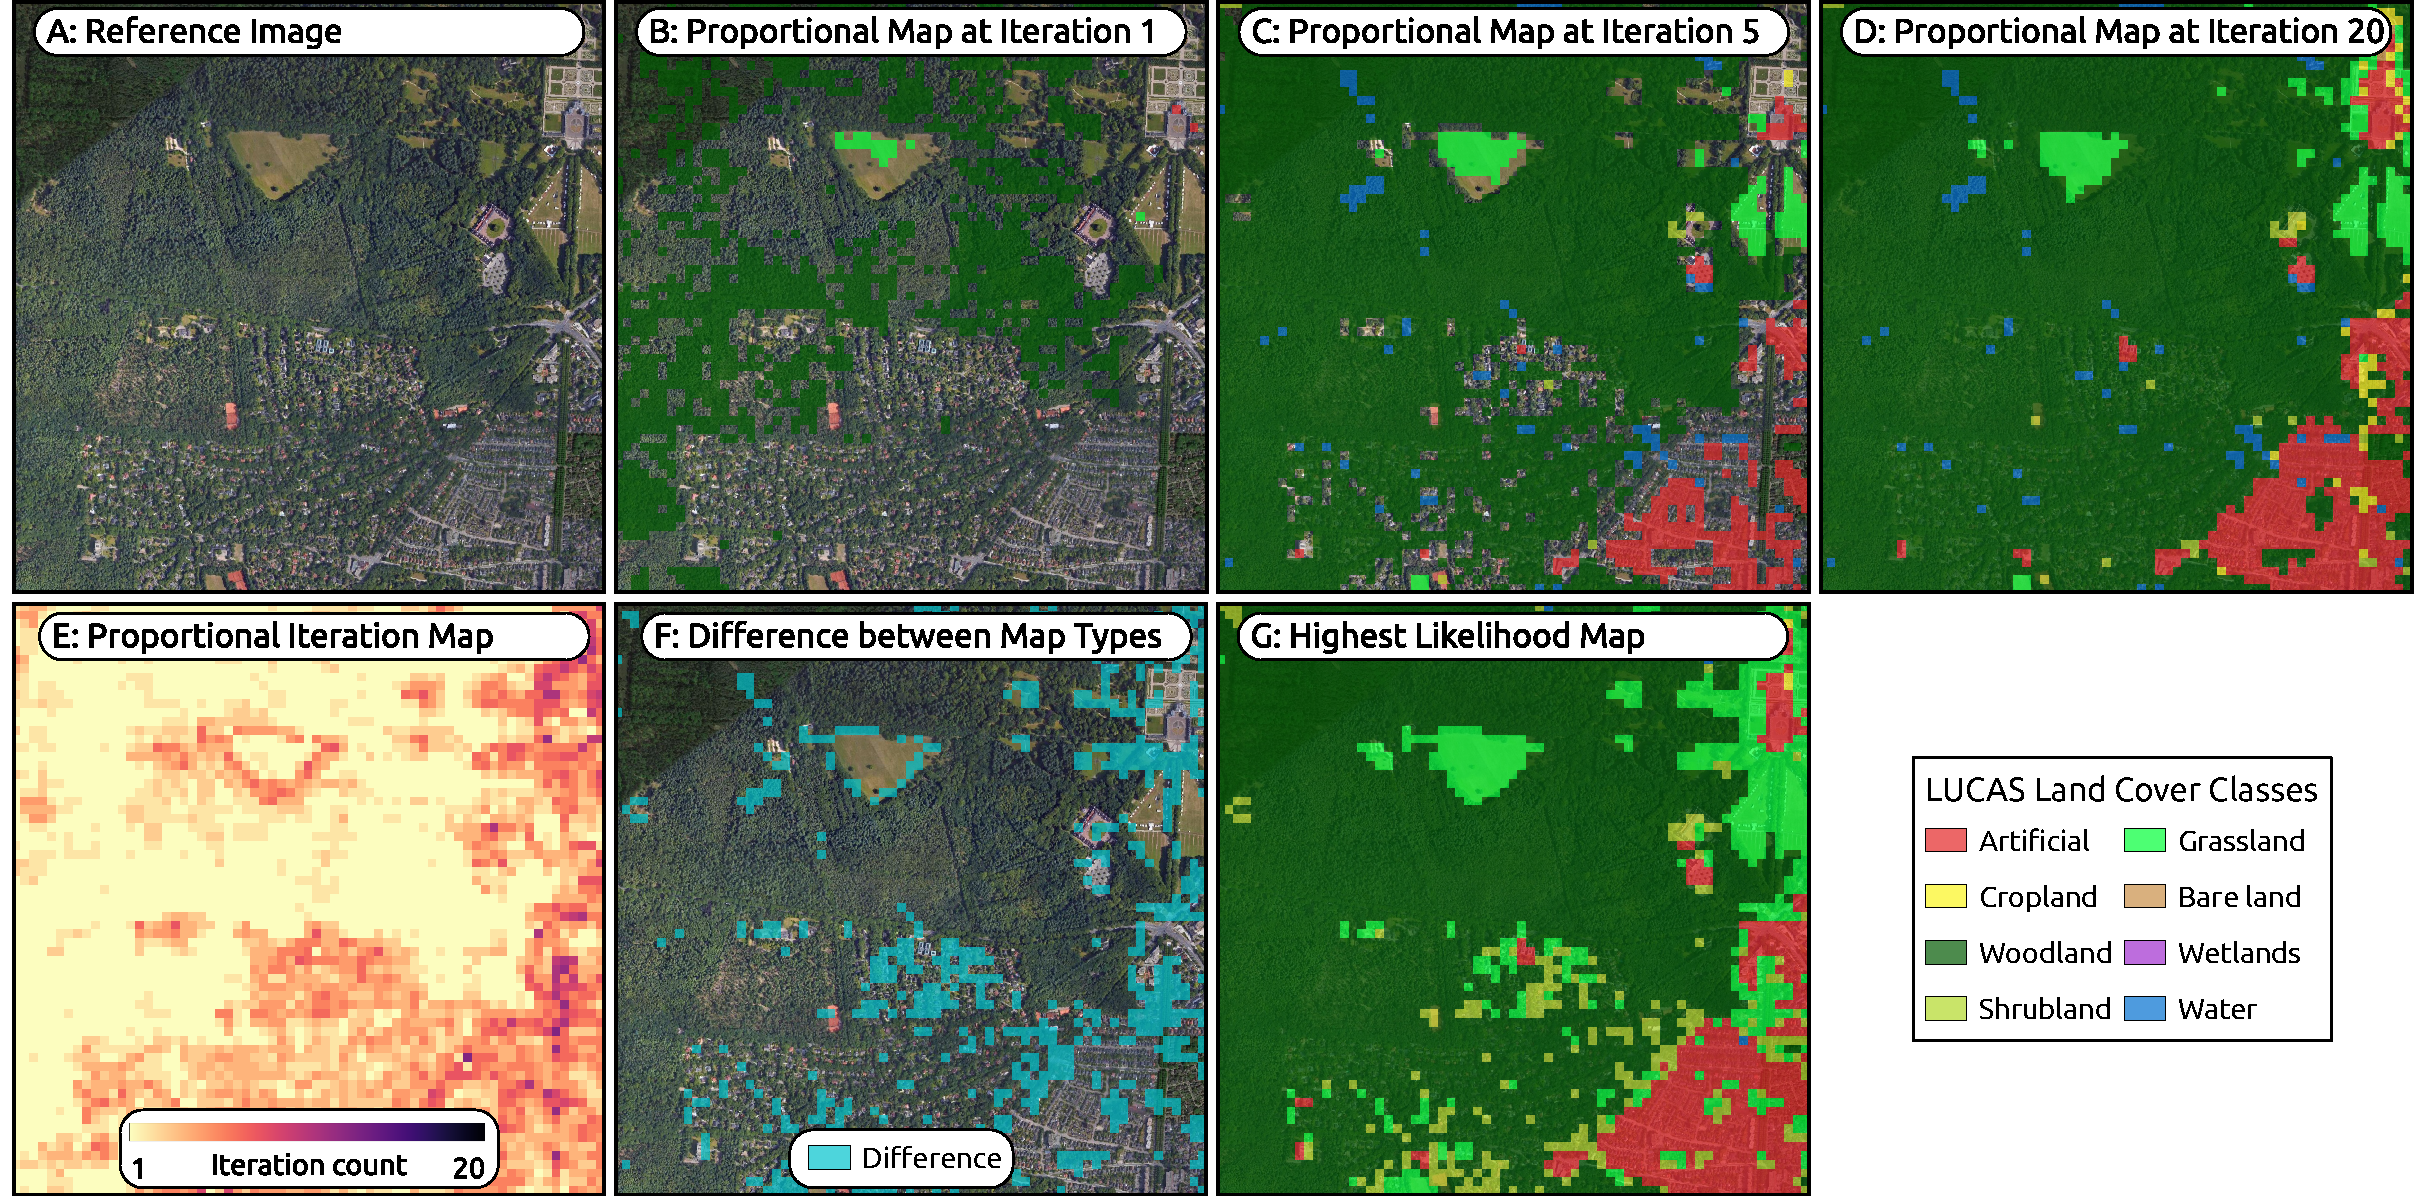
\includegraphics[width=\linewidth]{figs_04/fig5_example.pdf}
        \caption{Example of the IMP iterative classification process and comparison to highest likelihood classification, using the northwestern outskirts of Apeldoorn, the Netherlands. A: high-resolution reference imagery from Google Earth; B-D: classifications over subsequent iterations, identified in E; F: differences between  the proportional map and the highest likelihood map; G: the highest likelihood map itself.}
        \label{fig:map_example}
    \end{figure}

    A complete overview of the area estimates by Eurostat and mapped area per country, year, class, model type, and map type is included in ~\ref{appendix:full_area_results}. Almost all proportional maps had pixel proportions that fell within the confidence intervals of the Eurostat-derived area estimate. Only some maps derived from probabilities predicted by local models had class proportions that were outside the confidence intervals of the Eurostat area estimates. The only case of underrepresentation was \textit{Bare Land} in the maps derived from probabilities predicted by the local model for Luxembourg, as this class was not represented in the training data. Also in Luxembourg, Woodland was overrepresented by the local model by an average of 0.03 percent above the upper bound of the Eurostat-supplied confidence interval. Both issues are likely due to the fact that Luxembourg's local model was trained on a relatively small dataset compared to the other models, as no under- or overrepresentation occurred in proportional maps derived from probabilities produced by the general model.

    The \textit{Artificial} class was overrepresented in the 2012 map of Germany by 0.04 percent of the upper bound, and finally, the \textit{Shrubland} class was overrepresented in the 2009 map of Czechia by 11 percent. This is the biggest percentual error in all proportional maps, and constitutes a representation of 0.87 percent of Czechia's surface instead of the 0.69 percent estimated by Eurostat, with an upper confidence bound of 0.78 percent. This relatively large overrepresentation was caused after the final iteration, where remaining gaps in the map were filled with the highest likelihood class. These gaps were assigned to \textit{Grassland} and \textit{Shrubland}, for which more pixels were available with higher probabilities. Fig.~\ref{fig:fill_by_iterations} shows how the iterative classification, or 'filling' of the 2009 map of Czechia proceeded. The general behavior of each class is similar to those observed in other countries and years, but not every class approaches the area estimate at the same rate, with \textit{Woodland} reaching the confidence interval at iteration 8, and \textit{Grassland} at iteration 19.
    We observed a similar pattern in other maps: More gaps remained at the final iteration when there was a relatively small surplus of pixels with predicted probabilities for each class. Generally, classes for which there was a low number of pixels with any probability compared to their proportion according to the Eurostat estimate were classified less accurately, and in proportions that less closely matched the Eurostat estimates.
    Predictions by the general model tended to have probabilities for more different classes in each pixel, especially for rarer classes. Fig.~\ref{fig:probability_pixels} shows this for predictions for the Netherlands in 2009. Both models predicted probabilities above zero for \textit{Cropland} and \textit{Grassland} on a large number of pixels compared to their prevalence as estimated by Eurostat, but the local model barely predicted enough pixels for \textit{Bare Land}, and an insufficient amount for \textit{Water}. While the general model predicted a smaller surplus of pixels with probability above zero for Artificial and Woodland, it predicted surpluses for each class. The comparison of Eurostat estimates and counts based on classification in \ref{appendix:full_area_results} show that proportional maps based on probabilities predicted by the general model matched the Eurostat estimates more closely than those based on probabilities predicted by the local model.
    
    \begin{figure}[H]
        \centering
        \includegraphics[width=\linewidth]{figs_04/fig6_fill_by_iterations.pdf}
        \caption{Percentage of map area filled per iteration of the IMP algorithm, for the map of Czechia for 2009. Each line with dots indicates the percentage of area assigned to each LUCAS land cover class at each iteration. The dashed lines indicate the mean area estimated by Eurostat, with the lighter-colored area around each dashed line indicating the accompanying confidence interval.}
        \label{fig:fill_by_iterations}
    \end{figure}

    \begin{figure}[H]
        \vspace*{-4cm}
        \centering
        \begin{subfigure}[b]{\textwidth}
            \centering
            \caption{Local Model}\includegraphics[width=\textwidth]{figs_04/fig7a_probability_pixels_NL_local.pdf}
            \label{fig:probability_pixels_local}
            % \hspace{-0.9em}       
        \end{subfigure}
        \begin{subfigure}[b]{\textwidth}
           \centering
           \caption{General Model}
           \includegraphics[width=\textwidth]{figs_04/fig7b_probability_pixels_NL_general.pdf}
           \label{fig:probability_pixels_general}   
        \end{subfigure}
        % \vspace*{-0.75cm}
        
        \caption{Percentage of pixels for which any probability above zero was predicted per class, compared to the proportion of that class according to the Eurostat area estimate used to create proportional maps of the Netherlands in 2009. Note that the general model predicted a surplus of probabilities above zero for each class, while the local model did not predict probabilities above zero in enough pixels for \textit{Water}.}
        \label{fig:probability_pixels}
    \end{figure}



    \subsection{Accuracy assessment}
    
    F1-scores calculated by overlaying the highest likelihood and proportional maps of 2009, 2012, 2015 and 2018 on LUCAS points of matching years and the maps of 2017 on S2GLC points show (see Fig.~\ref{fig:f1}) the accuracy of proportional maps tended to be higher or equal to the accuracy of highest likelihood maps. The difference between highest likelihood maps and proportional maps created from the same predicted probabilities is more pronounced on maps created by the general model, which was trained on the entire training dataset. On average across all mapped years (see table \ref{tab:f1_scores}, proportional maps were more accurate than highest likelihood maps in most cases. Proportional maps consistently achieved a weighted F1-score above 0.7 on LUCAS points, and above 0.85 on S2GLC points. Fig.~\ref{fig:precision} shows that the highest likelihood maps generally had higher precision (User's accuracy) than proportional maps, while Fig.~\ref{fig:recall} shows that proportional maps generally had higher recall (Producer's accuracy). This sacrifice of precision for gains in recall can explain the noted increase in F1-score. Note that we use the \textit{weighted} precision and recall metrics to give equal importance to the performance of every class. 
    
    As shown in Fig.~\ref{fig:quantity_disagreement}, the proportional maps had a lower quantity disagreement than the maximum likelihood maps, reducing it to near-zero in most cases. It also shows that maximum likelihood maps based on probabilities predicted by local models tended to be more accurate than those based on probabilities predicted by the general model.

    \begin{table}[H]
    \caption{Comparison of F1-scores for different countries, validation datasets, and model types. The table presents the F1-scores for both highest likelihood and proportional maps across five countries, using two validation datasets (S2GLC and LUCAS) and two model types (local and general). The "Difference" column quantifies the difference in F1-scores between the highest likelihood and proportional maps. Note that the LUCAS values are averages of the 4 years that were mapped and validated: 2009, 2012, 2015 and 2018.}
    \centering
    \label{tab:f1_scores}
    \begin{tabular}{c|c|c|p{2.1cm}|p{2.12cm}|p{2cm}}
    Country & Dataset & Model Type & \multicolumn{3}{c}{F1-score} \\
    \cline{4-6}
           &         &            & Proportional & Highest Likelihood & Difference \\
    \hline
    \multirow{4}{*}{NL} & \multirow{2}{*}{S2GLC} & local & 0.85 & 0.86 & -0.01 \\
                        &                        & general & 0.86 & 0.80 & 0.06 \\
                        & \multirow{2}{*}{LUCAS} & local & 0.71 & 0.72 & -0.01 \\
                        &                        & general & 0.73 & 0.67 & 0.06 \\
    \hline
    \multirow{4}{*}{LU} & \multirow{2}{*}{S2GLC} & local & 0.95 & 0.98 & -0.03 \\
                        &                        & general & 0.97 & 0.91 & 0.06 \\
                        & \multirow{2}{*}{LUCAS} & local & 0.75 & 0.73 & 0.02 \\
                        &                        & general & 0.73 & 0.68 & 0.05 \\
    \hline
    \multirow{4}{*}{DE} & \multirow{2}{*}{S2GLC} & local & 0.94 & 0.93 & 0.01 \\
                        &                        & general & 0.93 & 0.83 & 0.10 \\
                        & \multirow{2}{*}{LUCAS} & local & 0.77 & 0.77 & 0.00 \\
                        &                        & general & 0.76 & 0.70 & 0.06 \\
    \hline
    \multirow{4}{*}{BE} & \multirow{2}{*}{S2GLC} & local & 0.90 & 0.87 & 0.03 \\
                        &                        & general & 0.92 & 0.87 & 0.05 \\
                        & \multirow{2}{*}{LUCAS} & local & 0.71 & 0.71 & 0.00 \\
                        &                        & general & 0.72 & 0.70 & 0.02 \\
    \hline
    \multirow{4}{*}{CZ} & \multirow{2}{*}{S2GLC} & local & 0.94 & 0.91 & 0.03 \\
                        &                        & general & 0.96 & 0.88 & 0.08 \\
                        & \multirow{2}{*}{LUCAS} & local & 0.78 & 0.78 & 0.00 \\
                        &                        & general & 0.78 & 0.73 & 0.05 \\
    \end{tabular}
    \end{table}




    \begin{figure}[H]
        \centering
        \includegraphics[width=\linewidth]{figs_04/fig8_jointplot_F1.pdf}
        \caption{Weighted F1-score of the land cover maps classified with maximum likelihood (X-axis) and the iterative mapping (Y-axis), validated on LUCAS and S2GLC reference data. Maps based on probabilities predicted by the general model are shown in blue, while maps based on probabilities predicted by local models are shown in orange. The boxplots at the top and right summarize the F1-scores of maximum likelihood and proportional classification, respectively. The diagonal reference line shows where the F1-score would be equal, while the horizontal and vertical line represent the average across all F1-scores. Points above the diagonal reference line indicate maps where proportional maps were more accurate. 
        In most cases, proportional maps had higher F1-scores than maximum likelihood maps. This difference was generally larger when using probabilities predicted by the general model, although maps based on predictions by local models were more accurate on average.}
        \label{fig:f1}
    \end{figure}

    \begin{figure}[H]
        \centering
        \includegraphics[width=\linewidth]{figs_04/fig9_jointplot_precision.pdf}
        \caption{Weighted precision (User's accuracy) of the land cover maps classified with maximum likelihood (X-axis) and the iterative mapping (Y-axis), validated on LUCAS and S2GLC reference data. Maps based on probabilities predicted by the general model are shown in blue, while maps based on probabilities predicted by local models are shown in orange. The boxplots at the top and right summarize the precision of maximum likelihood and proportional classification, respectively. The diagonal reference line shows where the F1-score would be equal, while the horizontal and vertical line represent the average across all precision scores. Points above the diagonal reference line indicate maps where proportional maps were more precise. 
        Note that proportional maps generally had a lower precision than maximum likelihood maps, and that this difference was bigger for maps based on probabilities predicted by local models.}
        \label{fig:precision}
    \end{figure}

    \begin{figure}[H]
        \centering
        \includegraphics[width=\linewidth]{figs_04/fig10_jointplot_recall.pdf}
        \caption{Weighted recall (Producer's accuracy) of the land cover maps classified with maximum likelihood (X-axis) and the iterative mapping (Y-axis), validated on LUCAS and S2GLC reference data. Maps based on probabilities predicted by the general model are shown in blue, while maps based on probabilities predicted by local models are shown in orange. The boxplots at the top and right summarize the recall of maximum likelihood and proportional classification, respectively. The diagonal reference line shows where the F1-score would be equal, while the horizontal and vertical line represent the average across all recall scores. Points above the diagonal reference line indicate maps where proportional maps had a higher recall. 
        Observations include: 1) Proportional class maps generally exhibit a marginally higher F1-score, 2) The range of quantity error for proportional class maps narrow compared to highest probability class maps, and 3) Highest probability maps generated by the general model were less accurate in terms of both quantity and allocation disagreement than those generated by local models.}
        \label{fig:recall}
    \end{figure}

    \begin{figure}[H]
    \vspace{-2cm}
        \centering
        \includegraphics[width=\linewidth]{figs_04/fig11_jointplot_area_percent_error.pdf}
        \caption{Class-wise allocation disagreement of maximum likelihood (X-axis) and proportional (Y-axis) maps based on probabilities predicted by the general model (blue) and local models (orange). Allocation disagreement is quantified as area percent error: the percent point difference between the target area estimate and the amount of pixels classified on the map. Note that proportional maps had errors close to zero, with the exception of Luxembourg (indicated with $+$), and that highest likelihood maps based on probabilities predicted by local models had lower quantity disagreement than those based on predictions by the general model.}
        \label{fig:quantity_disagreement}
    \end{figure}
    
\section{Discussion}

    \subsection{Algorithm design and performance}

        We found that IMP yielded higher accuracy compared to highest probability class assignment. 
    
        Where the use of prior probabilities to adjust classification thresholds such as summarized by \citet{mingguo2009effect} does not guarantee  method proposed by \citep{horvath2021comparison} leaves considerable gaps due to overlapping 'best probability' pixels for several classes, our iterative approach with a decaying threshold minimizes this problem by classifying the best pixels for every class first. Any remaining unclassified pixels can be filled in with the highest likelihood class without severely affecting the distribution of classes. The number of iterations can be increased to improve convergence to area estimates, which might be needed if there are relatively few pixels with probabilities for one or more classes. Using models that push probability mass away from 0 and 1 like boosting \citep{niculescu2005predicting}, as was used in this work, may play a role as well.
    
        We did not expect the proportional maps to be consistently either equally or more accurate than those created by highest likelihood classification. A possible explanation for this improvement in accuracy is that by forcing the classification to be stratified according to an accurate area estimate, we reduce the bias of the model. This is supported by the fact that the difference in accuracy between proportional and highest likelihood class maps was higher when using probabilities predicted by the general model: A general model, having been trained on a dataset that is less representative of any given country, is therefore likely to be more biased \citep{he2009learning}, which gives more space for the iterative algorithm to improve the map. This corresponds to claims by \citet{sales2022land} and \citet{kleinewillinghofer2022unbiased} that area estimates are better derived from predictions by models that were trained on datasets representative of the area of interest.

    \subsection{Limitations and potential improvements}

        While the proposed algorithm correctly mapped to area proportions in most attempts, this is not generally guaranteed. Experiments with different preprocessing workflows, model types, and parameters such as the number of iterations, suggested that the algorithm performs better in both quantity and allocation accuracy when, respectively, more pixels in the area of interest have a predicted probability for multiple classes (see Figs.\ref{fig:fill_by_iterations}~and~\ref{fig:probability_availability_pixels}), and when these probabilities are properly ranked within each class. We did not include these initial experiments for the sake of brevity, but this should be taken into account when applying our method to other probability predictions. Based on our omitted findings about the quantity of pixels with predicted probabilities for any given class, we expect techniques that push probability mass away from extreme values, such as label smoothing \citep{müller2020when} might help the algorithm converge to the area estimates, as more pixels will be available with probabilities for more classes. This might not lead to more accurate maps by itself, however. It is possible that accuracy of proportional maps could be increased by using probabilities that more closely meet the assumption that probabilities are properly ranked, such as those produced by Platt Scaling \citep{niculescu2005predicting}.

    \subsection{Potential applications}

        The primary purpose for which this algorithm was designed is to create, or update, land cover maps based on predicted probabilities, using a given area estimate. This area estimate can be derived from an external source, such as a sample-based measurement, like in the case of this study. However, the algorithm might also be used to update a map used to derive area estimates with post-stratification sampling \citep{olofsson2014good}, using the corrected area estimates and the original probabilities that were used to make the initial map. Besides this purpose, however, we suggest interested parties consider the following:

        Our results show that the single, bigger \textit{general model} was often less accurate when mapping a single area of interest than the \textit{local models} that were trained only on data from their corresponding country. However, this difference in accuracy disappeared in proportional maps, and the general model successfully detected a rare class that was not present in the training data for Luxembourg, whereas the local model simply skipped these classes.

        Additionally, the iterative nature of IMP enables the production of spatially explicit uncertainty assessments. Pixel-level uncertainty is useful because it can be propagated in spatial models that use land cover as a covariate \citep{herold2016toward}. During this study, we found that the pixels classified in earlier iterations have a higher validation allocation disagreement than those classified in later iterations (see Fig.~\ref{fig:f1_score_during_filling} for an example). It is therefore possible to calculate separate precision (User's accuracy) scores per class and per iteration, leading to a more fine-grained indicator of each pixel's reliability for decision makers or use in subsequent modeling. The combination these 'iteration maps' (see Fig.~\ref{fig:map_example}~E)  with the user's accuracy of each iteration needs further study. 

        \begin{figure}
            \vspace*{-4cm}
            \centering
            \begin{subfigure}[b]{0.82\textwidth}
            \centering
            \caption{Local Model}\includegraphics[width=\textwidth]{figs_04/fig12a_f1_during_filling_local.pdf}
            \label{fig:f1_filling_local}
            \hspace{-0.9em}
            
            \end{subfigure}
            
            \begin{subfigure}[b]{0.82\textwidth}
           \centering
           \caption{General Model}
           \includegraphics[width=\textwidth]{figs_04/fig12b_f1_during_filling_general.pdf}
           \label{fig:f1_filling_general}
           
        \end{subfigure}
            \vspace*{-0.75cm}
            \caption{Validation performance of proportional maps compared to the highest likelihood baseline. This example of the weighted F1 score of the partially filled-in map during each iteration of IMP, and a comparison with the weighted F1-score of the highest likelihood map when derived from probabilities predicted by the local (a) and general (b) model. The lines represent validations of all maps of Czechia. Note that the pixels classified at early iterations achieve a higher score, and that the score gradually decreases as a greater number of pixels is classified, stabilizing at or above baseline established by highest likelihood maps.}
            \label{fig:f1_score_during_filling}
        \end{figure}
    
        Furthermore, it is possible that our proposed algorithm might improve the temporal consistency of land cover classification, leading to better land cover change mapping. Due to variations in satellite reflectance per mapped time period, spurious changes are often included in land cover change maps that do not implement proper post-processing techniques. While many such techniques already exist, they often rely on contiguous time series of predictions or are computationally intensive. Our proposed algorithm does not have these limitations, only requiring an up-to-date area estimate of each year, or an interpolation such as the one used to make maps of the year 2017 in this study. If further research indicates that the algorithm can reduce spurious change, it would therefore be a useful addition to the existing methods.
        
        Lastly, during this study it became clear that the method might be suitable for more than only making maps whose proportions match area estimates. The observed improvement in accuracy of proportional maps output by IMP over highest likelihood classification suggests that forcibly improving quantity disagreement with posterior quantity estimates can improve allocation disagreement to a certain extent. This means that IMP could be used to validate area estimates themselves. When provided with 1) a validation dataset that was not used in the area estimation process and suitable for the mapped resolution (such as the S2GLC points in this study), 2) predicted probabilities of sufficient quality, and 3) multiple area estimates, the best area estimate should lead to the most accurate proportional map possible. Exploring this further was beyond the scope of this study but may prove a promising use case.

\section{Conclusion}

    We present an algorithm that can transform predicted probabilities by a given machine learning model into maps whose class proportions match area estimates. Our validation on two independent test datasets (LUCAS and S2GLC points) across five years and five countries show that these maps were also equally, if not more, accurate than maps classified according to the maximum probability per pixel. In our experiments, this increase in accuracy was achieved by sacrificing some degree of precision (User's accuracy) for relatively larger gains in recall (Producer's accuracy). Because pixels classified at each iteration have different precision and recall values, the iteration at which a pixel was classified can be used to approximate pixel-wise uncertainty. 
    IMP greatly improves the accuracy of models trained on a bigger, but imbalanced, training dataset. This means that it can be used to optimize predictions by big models to local contexts if reliable area estimates are available. This offers potential for the increasing number of global and continental-scale maps which are trained on a rich feature space and achieve high overall accuracy, but have also been criticized for their relatively low accuracy and/or usefulness at more local scales. By negating the bias from large scale models, IMP can therefore contribute to make accurate and useful maps of smaller regions. This, combined with the potential to generate pixel-based error estimates, suggests that IMP can be a valuable tool for decision makers and other stakeholders.

\section{Data Availability}
The 400 predicted probability layers, 50 highest likelihood class maps, and 50 proportional class maps, are available on zenodo at https://zenodo.org/records/10641340. This download is accompanied by the used area estimates, and a script that produces proportional maps.

\section{Appendices}

    \subsection*{Training point filtering}
    \label{tab:corine_filtering}
    \begin{table}[H]
    \caption{Point filtering rules per class used to remove potential label errors from the CORINE centroids before using them as training data, as well as the number of points that resulted.}
    
    \begin{tabular}{lrlrr}
    \hline
    LUCAS class    & Condition  & dataset                                      & Source & Removed \\
    \hline
    Artificial     & \verb|>| 150    & OSM Buildings / Cop Imp.  & \citep{witjes2022spatiotemporal}       & 68,444  \\
    Artificial     & \verb|<| 50     & OSM buildings / Cop Imp.  & \citep{witjes2022spatiotemporal}       & 333,526 \\
    Non-Artificial & \verb|> 50 <| 150 & OSM buildings / Cop Imp.  & \citep{witjes2022spatiotemporal}       & 9,594   \\
    Non-Artificial & \verb|>| 30     & Rasterized OSM Roads                       & \citep{witjes2022spatiotemporal}       & 161,576 \\
    Non-Artificial & \verb|>| 30     & Rasterized OSM Railroads                   & \citep{witjes2022spatiotemporal}       & 2,759   \\
    Woodland       & \verb|<| 1      & Cop Tree Cover                      &   \citep{copernicus2023hrl}      & 62,731  \\
    Shrubland      & \verb|>| 50     & Cop Tree Cover                      &  \citep{copernicus2023hrl}       & 121,464 \\
    Shrubland      & \verb|>| 50     & Cop Grassland                       &  \citep{copernicus2023hrl}       & 48,734  \\
    Grassland      & \verb|<| 1      & Cop Grassland                       &  \citep{copernicus2023hrl}       & 174,616 \\
    Grassland      & \verb|>| 30     & Cop Tree Cover                      &  \citep{copernicus2023hrl}       & 48,443  \\
    Bare Land      & \verb|>| 1      & Cop Tree Cover                      &  \citep{copernicus2023hrl}       & 16,156  \\
    Bare Land      & \verb|>| 1      & Cop Grassland                       &  \citep{copernicus2023hrl}       & 11,052  \\
    Wetlands       & \verb|<| 1      & Cop Temp and Perm Wetness &  \citep{copernicus2023hrl}       & 7,973   \\
    Water          & \verb|<| 50     & Cop Permanent Water                 &  \citep{copernicus2023hrl}       & 9,511 \\
    \hline
    \end{tabular}
    \end{table}
    
\subsection*{IMP Algorithm in pseudocode}
    \label{alg:imp}
    \newcommand{\lbox}[2]{\parbox[t]{\dimexpr 0.9\linewidth-#1em}{#2 \strut}}

    \begin{algorithm}[H]
    \caption{Iterative Mapping of Probabilities}
    
    \begin{algorithmic}[1]
    \Statex \textbf{Input:} 
    \Statex \textbullet~$P$, predicted probabilities for each class $C$
    \Statex \textbullet~$E$, the target area estimate 
    \Statex \textbullet~$I$, the number of iterations
    \Statex \textbf{Output:}
    \Statex \textbullet~$M$, the land cover map whose class proportions should match $E$.
    
    \noindent\rule[0.5ex]{\linewidth}{1pt}
    \Statex \textbf{1:} Initialize the empty output map $M$
    \Statex \textbf{2:} \textbf{for} iteration $i = 1$ to $I+1$ \textbf{do}
        \Statex\hspace*{1em} \textbf{2.1} \lbox{1}{Set ratio $r_i$ to $\frac{i}{I}$}
        \Statex\hspace*{1em} \textbf{2.2} \lbox{1}{\textbf{for} each $C$ \textbf{do}}
            \Statex\hspace*{2em} \textbf{2.2.1} \lbox{2}{$E_C$ = The target number of pixels of $C$ in the output $M$ according to $E$}
            \Statex\hspace*{2em} \textbf{2.2.2} \lbox{2}{$M_{Ci}$ = Number of pixels in $M$ already classified as $C$ at $i$}
            \Statex\hspace*{2em} \textbf{2.2.3} \lbox{2}{$N_{Ci}$ = Number of pixels that must still be classified as $C$ to match $E_C$}
            \Statex\hspace*{2em} \textbf{2.2.4} \lbox{2}{$P_C$ = All pixels in $P$ with probability for $C$ above 0}
            \Statex\hspace*{2em} \textbf{2.2.5} \lbox{2}{$P_{Ci}$ = All unclassified pixels in $P_C$}
            \Statex\hspace*{2em} \textbf{2.2.6} \lbox{2}{$E_{Ci}$ = Number of pixels to classify in $i$ = $N_C \times r_i$}
            \Statex\hspace*{2em} \textbf{2.2.7} \lbox{2}{$Q$ = the top $\frac{E_{Ci}}{P_{Ci}}$-th percentile of $P_{Ci}$}
            \Statex\hspace*{2em} \textbf{2.2.8} \lbox{2}{$P_Q$ = The lowest probability among pixels in $Q$}
            \Statex\hspace*{2em} \textbf{2.2.9} \lbox{2}{$N_{CQ}$ = Number of pixels in $P$ with probability values  $\ge{} P_Q$ for $C$.}
            \Statex\hspace*{2em} \textbf{2.2.10} \lbox{2}{\textbf{if} $N_{CQ} > N_{Ci}$ \textbf{do}}
                \Statex\hspace*{3em}\textbullet~\lbox{3}{Select all pixels with probability $\ge{} P_Q + 1$ \& update $N_{CQ}$}
                \Statex\hspace*{3em}\textbullet~\lbox{3}{Randomly sample $N_{CQ}-N_{Ci}$ pixels with probability $P_Q$}
                \Statex\hspace*{3em}\textbullet~\lbox{3}{Classify both pixel groups as $C$}                
            \Statex\hspace*{2em} \textbf{else}
                \Statex\hspace*{3em}\textbullet~\lbox{3}{Classify all pixels in $P_{Ci}$ with probability $\ge{} P_Q$ as $C$.}
    \Statex \textbf{3:} \lbox{0}{Classify all remaining unclassified pixels using highest likelihood classification.}
    \end{algorithmic}
    \end{algorithm}

    \subsection*{Full area results}
    \label{appendix:full_area_results}
    This appendix shows the area per land cover as estimated by Eurostat, predicted by both the country's local model and the general model, and processed into a hard-class map by both highest likelihood classification and iterative mapping of probabilities. The 'Best' columns show which combination of model type and mapping type resulted in a mapped area that most closely matched the mean estimated by Eurostat. The Eurostat 'Min' and 'Max' columns are the estimated mean minus and plus the reported variance of the estimate; these indicate the range that should ideally contain the mapped area. 
    
    
    
    \subsubsection{Belgium}
    Proportional maps of Belgium consistently matched Eurostat area estimates more closely than highest likelihood maps. Out of 5 years for 8 classes, classes mapped from predictions by general models matched Eurostat estimates more closely than those made from predictions by local models 8 times, while classes mapped from local model predictions had a closer match 6 times.
    \begin{table}[H]
    \centering
    \caption{Land cover area estimated by Eurostat and classified by both model (local and general) and map (highest likelihood and proportional) types for BE in 2009.}
    
    \begin{tabular}{r|rrr|rr|rr|rr}
    \toprule
    {} & \multicolumn{3}{|c}{Eurostat} & \multicolumn{2}{|c}{Highest Likelihood} & \multicolumn{2}{|c}{Proportional} & \multicolumn{2}{|c}{Best} \\
    {} &      Min &   Mean &    Max &              Local & General &        Local & General &  Model &    Map \\
    \midrule
    Artificial &     9.39 &   9.92 &  10.45 &              16.32 &   11.58 &         9.92 &    9.95 &  Local &  Prop. \\
    Cropland   &    26.05 &  26.72 &  27.38 &              20.41 &   19.16 &        26.72 &   26.72 &    Tie &  Prop. \\
    Woodland   &    23.88 &  24.54 &   25.2 &               25.0 &   21.31 &        24.54 &   24.54 &    Tie &  Prop. \\
    Shrubland  &     0.79 &   0.94 &   1.09 &               0.96 &    3.27 &         0.94 &    0.96 &  Local &  Prop. \\
    Grassland  &    34.37 &  35.29 &   36.2 &              36.82 &   43.51 &        35.27 &   35.23 &  Local &  Prop. \\
    Bare land  &      0.9 &   1.13 &   1.37 &                0.0 &    0.13 &         1.14 &    1.14 &    Tie &  Prop. \\
    Wetlands   &     0.05 &   0.07 &   0.09 &                0.0 &    0.08 &         0.08 &    0.08 &    Tie &    Tie \\
    Water      &     1.23 &    1.4 &   1.57 &               0.49 &    0.95 &          1.4 &     1.4 &    Tie &  Prop. \\
    \bottomrule
    \end{tabular}
    \end{table}
    
    \begin{table}[H]
    \centering
    \caption{Land cover area estimated by Eurostat and classified by both model (local and general) and map (highest likelihood and proportional) types for BE in 2012.}
    
    \begin{tabular}{r|rrr|rr|rr|rr}
    \toprule
    {} & \multicolumn{3}{|c}{Eurostat} & \multicolumn{2}{|c}{Highest Likelihood} & \multicolumn{2}{|c}{Proportional} & \multicolumn{2}{|c}{Best} \\
    {} &      Min &   Mean &    Max &              Local & General &        Local & General &    Model &    Map \\
    \midrule
    Artificial &    10.33 &  10.84 &  11.35 &              16.15 &   11.48 &        10.85 &   10.85 &      Tie &  Prop. \\
    Cropland   &     28.7 &  29.44 &  30.18 &              19.95 &    16.9 &        29.44 &   29.42 &    Local &  Prop. \\
    Woodland   &    23.75 &  24.31 &  24.87 &              25.23 &    21.2 &        24.31 &   24.31 &      Tie &  Prop. \\
    Shrubland  &     0.74 &   0.85 &   0.97 &               1.39 &    3.83 &         0.86 &    0.86 &      Tie &  Prop. \\
    Grassland  &    31.08 &  31.98 &  32.88 &               36.7 &   45.42 &        31.96 &   31.98 &  General &  Prop. \\
    Bare land  &      0.7 &   0.81 &   0.91 &                0.0 &    0.11 &         0.81 &    0.81 &      Tie &  Prop. \\
    Wetlands   &     0.28 &   0.34 &    0.4 &                0.0 &    0.12 &         0.35 &    0.35 &      Tie &  Prop. \\
    Water      &     1.24 &   1.43 &   1.62 &               0.58 &    0.94 &         1.43 &    1.43 &      Tie &  Prop. \\
    \bottomrule
    \end{tabular}
    \end{table}
    
    \begin{table}[H]
    \centering
    \caption{Land cover area estimated by Eurostat and classified by both model (local and general) and map (highest likelihood and proportional) types for BE in 2015.}
    
    \begin{tabular}{r|rrr|rr|rr|rr}
    \toprule
    {} & \multicolumn{3}{|c}{Eurostat} & \multicolumn{2}{|c}{Highest Likelihood} & \multicolumn{2}{|c}{Proportional} & \multicolumn{2}{|c}{Best} \\
    {} &      Min &   Mean &    Max &              Local & General &        Local & General &    Model &    Map \\
    \midrule
    Artificial &     10.9 &  11.39 &  11.88 &              14.49 &   10.59 &         11.5 &   11.39 &  General &  Prop. \\
    Cropland   &     28.2 &  28.54 &  28.88 &               21.9 &   19.75 &        28.54 &   28.53 &    Local &  Prop. \\
    Woodland   &    24.42 &  24.67 &  24.92 &              25.21 &   21.94 &        24.68 &   24.67 &  General &  Prop. \\
    Shrubland  &     1.56 &   1.63 &    1.7 &               1.14 &    2.94 &         1.63 &    1.63 &      Tie &  Prop. \\
    Grassland  &     30.4 &  31.02 &  31.64 &              36.67 &   43.57 &        30.89 &   31.03 &  General &  Prop. \\
    Bare land  &     0.75 &   0.83 &   0.91 &                0.0 &    0.11 &         0.83 &    0.83 &      Tie &  Prop. \\
    Wetlands   &     0.27 &   0.47 &   0.67 &                0.0 &    0.08 &         0.47 &    0.47 &      Tie &  Prop. \\
    Water      &     1.29 &   1.45 &   1.61 &               0.59 &    1.01 &         1.46 &    1.46 &      Tie &  Prop. \\
    \bottomrule
    \end{tabular}
    \end{table}
    
    \begin{table}[H]
    \centering
    \caption{Land cover area estimated by Eurostat and classified by both model (local and general) and map (highest likelihood and proportional) types for BE in 2017.}
    
    \begin{tabular}{r|rrr|rr|rr|rr}
    \toprule
    {} & \multicolumn{3}{|c}{Eurostat} & \multicolumn{2}{|c}{Highest Likelihood} & \multicolumn{2}{|c}{Proportional} & \multicolumn{2}{|c}{Best} \\
    {} &      Min &   Mean &    Max &              Local & General &        Local & General &    Model &    Map \\
    \midrule
    Artificial &    11.13 &  11.62 &  12.12 &              14.75 &   10.74 &        11.76 &   11.63 &  General &  Prop. \\
    Cropland   &    28.53 &  28.89 &  29.26 &              19.49 &   18.67 &         28.9 &   28.88 &    Local &  Prop. \\
    Woodland   &     25.6 &  25.86 &  26.12 &              23.47 &   19.67 &        25.86 &   25.86 &      Tie &  Prop. \\
    Shrubland  &     1.33 &   1.39 &   1.45 &               1.13 &    3.24 &         1.39 &    1.39 &      Tie &  Prop. \\
    Grassland  &    28.51 &  29.11 &  29.71 &              40.63 &   46.39 &        28.96 &   29.11 &  General &  Prop. \\
    Bare land  &     1.33 &   1.44 &   1.55 &                0.0 &    0.11 &         1.45 &    1.45 &      Tie &  Prop. \\
    Wetlands   &     0.31 &   0.46 &    0.6 &                0.0 &    0.16 &         0.46 &    0.46 &      Tie &  Prop. \\
    Water      &      1.1 &   1.22 &   1.34 &               0.54 &    1.02 &         1.23 &    1.23 &      Tie &  Prop. \\
    \bottomrule
    \end{tabular}
    \end{table}
    
    \begin{table}[H]
    \centering
    \caption{Land cover area estimated by Eurostat and classified by both model (local and general) and map (highest likelihood and proportional) types for BE in 2018.}
    
    \begin{tabular}{r|rrr|rr|rr|rr}
    \toprule
    {} & \multicolumn{3}{|c}{Eurostat} & \multicolumn{2}{|c}{Highest Likelihood} & \multicolumn{2}{|c}{Proportional} & \multicolumn{2}{|c}{Best} \\
    {} &      Min &   Mean &    Max &              Local & General &        Local & General &    Model &    Map \\
    \midrule
    Artificial &    11.25 &  11.74 &  12.24 &              15.07 &   10.72 &        11.79 &   11.75 &  General &  Prop. \\
    Cropland   &    28.69 &  29.07 &  29.44 &               22.4 &   21.55 &        28.99 &   29.05 &  General &  Prop. \\
    Woodland   &    26.19 &  26.46 &  26.72 &              25.02 &   21.66 &        26.46 &   26.46 &      Tie &  Prop. \\
    Shrubland  &     1.21 &   1.27 &   1.33 &               1.39 &    3.41 &         1.28 &    1.28 &      Tie &  Prop. \\
    Grassland  &    27.56 &  28.15 &  28.74 &              35.54 &   41.43 &        28.16 &   28.16 &      Tie &  Prop. \\
    Bare land  &     1.63 &   1.75 &   1.87 &                0.0 &    0.12 &         1.76 &    1.76 &      Tie &  Prop. \\
    Wetlands   &     0.33 &   0.45 &   0.57 &                0.0 &    0.09 &         0.46 &    0.46 &      Tie &  Prop. \\
    Water      &     1.01 &   1.11 &   1.21 &               0.58 &    1.01 &         1.11 &    1.11 &      Tie &  Prop. \\
    \bottomrule
    \end{tabular}
    \end{table}
    
    \subsubsection{Czechia}
    Proportional maps of Czechia consistently matched Eurostat area estimates more closely than highest likelihood maps. Out of 5 years for 8 classes, classes mapped from predictions by general models matched Eurostat estimates more closely than those made from predictions by local models 4 times, while classes mapped from local model predictions had a closer match 9 times.
    
    \begin{table}[H]
    \centering
    \caption{Land cover area estimated by Eurostat and classified by both model (local and general) and map (highest likelihood and proportional) types for CZ in 2009.}
    
    \begin{tabular}{r|rrr|rr|rr|rr}
    \toprule
    {} & \multicolumn{3}{|c}{Eurostat} & \multicolumn{2}{|c}{Highest Likelihood} & \multicolumn{2}{|c}{Proportional} & \multicolumn{2}{|c}{Best} \\
    {} &      Min &   Mean &    Max &              Local & General &        Local & General &    Model &    Map \\
    \midrule
    Artificial &     4.05 &   4.26 &   4.47 &               4.41 &     4.0 &         4.31 &    4.27 &  General &  Prop. \\
    Cropland   &    33.16 &  33.63 &  34.11 &               31.7 &   26.96 &        33.64 &   33.56 &    Local &  Prop. \\
    Woodland   &    36.35 &   36.8 &  37.24 &              34.74 &   23.82 &         36.8 &    36.8 &      Tie &  Prop. \\
    Shrubland  &      0.6 &   0.69 &   0.78 &               1.77 &    7.78 &         0.87 &    0.69 &  General &  Prop. \\
    Grassland  &    21.77 &  22.26 &  22.75 &              26.28 &   36.44 &        22.02 &   22.33 &  General &  Prop. \\
    Bare land  &      0.7 &   0.81 &   0.92 &                0.0 &    0.05 &         0.81 &    0.81 &      Tie &  Prop. \\
    Wetlands   &     0.19 &   0.26 &   0.32 &               0.28 &    0.06 &         0.26 &    0.26 &      Tie &  Prop. \\
    Water      &     1.19 &   1.29 &   1.39 &               0.83 &    0.89 &          1.3 &     1.3 &      Tie &  Prop. \\
    \bottomrule
    \end{tabular}
    \end{table}
    
    \begin{table}[H]
    \centering
    \caption{Land cover area estimated by Eurostat and classified by both model (local and general) and map (highest likelihood and proportional) types for CZ in 2012.}
    
    \begin{tabular}{r|rrr|rr|rr|rr}
    \toprule
    {} & \multicolumn{3}{|c}{Eurostat} & \multicolumn{2}{|c}{Highest Likelihood} & \multicolumn{2}{|c}{Proportional} & \multicolumn{2}{|c}{Best} \\
    {} &      Min &   Mean &    Max &              Local & General &        Local & General &  Model &    Map \\
    \midrule
    Artificial &     4.21 &   4.41 &   4.61 &               4.42 &    4.13 &         4.41 &    4.41 &    Tie &  Prop. \\
    Cropland   &    32.21 &  32.84 &  33.46 &              30.03 &   25.35 &        32.79 &   32.75 &  Local &  Prop. \\
    Woodland   &     37.0 &  37.72 &  38.43 &              35.21 &   25.57 &        37.72 &   37.72 &    Tie &  Prop. \\
    Shrubland  &     0.67 &   0.78 &   0.89 &               1.63 &    6.43 &         0.79 &    0.79 &    Tie &  Prop. \\
    Grassland  &    20.95 &  21.99 &  23.02 &               27.6 &   37.47 &        22.02 &   22.06 &  Local &  Prop. \\
    Bare land  &      0.6 &    0.7 &   0.79 &                0.0 &    0.06 &          0.7 &     0.7 &    Tie &  Prop. \\
    Wetlands   &     0.14 &   0.18 &   0.21 &               0.25 &    0.06 &         0.18 &    0.18 &    Tie &  Prop. \\
    Water      &     1.14 &   1.39 &   1.65 &               0.86 &    0.95 &          1.4 &     1.4 &    Tie &  Prop. \\
    \bottomrule
    \end{tabular}
    \end{table}
    
    \begin{table}[H]
    \centering
    \caption{Land cover area estimated by Eurostat and classified by both model (local and general) and map (highest likelihood and proportional) types for CZ in 2015.}
    
    \begin{tabular}{r|rrr|rr|rr|rr}
    \toprule
    {} & \multicolumn{3}{|c}{Eurostat} & \multicolumn{2}{|c}{Highest Likelihood} & \multicolumn{2}{|c}{Proportional} & \multicolumn{2}{|c}{Best} \\
    {} &      Min &   Mean &    Max &              Local & General &        Local & General &    Model &    Map \\
    \midrule
    Artificial &     4.42 &   4.62 &   4.83 &               3.82 &    3.71 &         4.63 &    4.63 &      Tie &  Prop. \\
    Cropland   &    31.77 &  32.03 &  32.29 &              31.72 &   27.78 &        32.04 &   31.92 &    Local &  Prop. \\
    Woodland   &    37.27 &  37.53 &  37.79 &              34.64 &   26.23 &        37.53 &   37.53 &      Tie &  Prop. \\
    Shrubland  &     0.93 &    1.0 &   1.07 &               1.49 &    5.63 &         0.96 &     1.0 &  General &  Prop. \\
    Grassland  &    22.07 &  22.31 &  22.56 &              27.25 &   35.57 &        22.34 &    22.4 &    Local &  Prop. \\
    Bare land  &     0.81 &   0.87 &   0.92 &                0.0 &    0.06 &         0.87 &    0.87 &      Tie &  Prop. \\
    Wetlands   &     0.23 &   0.26 &   0.29 &               0.21 &    0.07 &         0.26 &    0.26 &      Tie &  Prop. \\
    Water      &     1.33 &   1.38 &   1.43 &               0.86 &    0.95 &         1.38 &    1.38 &      Tie &  Prop. \\
    \bottomrule
    \end{tabular}
    \end{table}
    
    \begin{table}[H]
    \centering
    \caption{Land cover area estimated by Eurostat and classified by both model (local and general) and map (highest likelihood and proportional) types for CZ in 2017.}
    
    \begin{tabular}{r|rrr|rr|rr|rr}
    \toprule
    {} & \multicolumn{3}{|c}{Eurostat} & \multicolumn{2}{|c}{Highest Likelihood} & \multicolumn{2}{|c}{Proportional} & \multicolumn{2}{|c}{Best} \\
    {} &      Min &   Mean &    Max &              Local & General &        Local & General &  Model &    Map \\
    \midrule
    Artificial &     4.32 &   4.46 &   4.59 &               4.22 &    3.91 &         4.46 &    4.46 &    Tie &  Prop. \\
    Cropland   &    32.93 &  33.17 &  33.41 &               30.9 &   27.57 &        33.17 &   33.12 &  Local &  Prop. \\
    Woodland   &    37.82 &  38.06 &  38.31 &              34.82 &   27.07 &        38.07 &   38.07 &    Tie &  Prop. \\
    Shrubland  &     0.94 &    1.0 &   1.06 &               1.11 &    4.36 &          1.0 &     1.0 &    Tie &  Prop. \\
    Grassland  &    20.64 &  20.86 &  21.08 &              27.87 &   36.04 &        20.84 &    20.9 &  Local &  Prop. \\
    Bare land  &     0.82 &   0.87 &   0.93 &                0.0 &    0.04 &         0.88 &    0.88 &    Tie &  Prop. \\
    Wetlands   &     0.27 &   0.29 &   0.32 &               0.19 &    0.06 &          0.3 &     0.3 &    Tie &  Prop. \\
    Water      &     1.24 &   1.29 &   1.33 &               0.89 &    0.96 &         1.29 &    1.29 &    Tie &  Prop. \\
    \bottomrule
    \end{tabular}
    \end{table}
    
    \begin{table}[H]
    \centering
    \caption{Land cover area estimated by Eurostat and classified by both model (local and general) and map (highest likelihood and proportional) types for CZ in 2018.}
    
    \begin{tabular}{r|rrr|rr|rr|rr}
    \toprule
    {} & \multicolumn{3}{|c}{Eurostat} & \multicolumn{2}{|c}{Highest Likelihood} & \multicolumn{2}{|c}{Proportional} & \multicolumn{2}{|c}{Best} \\
    {} &      Min &   Mean &    Max &              Local & General &        Local & General &  Model &    Map \\
    \midrule
    Artificial &     4.28 &   4.37 &   4.47 &               4.41 &    4.16 &         4.38 &    4.38 &    Tie &  Prop. \\
    Cropland   &     33.5 &  33.74 &  33.97 &              31.13 &   28.08 &        33.72 &   33.65 &  Local &  Prop. \\
    Woodland   &     38.1 &  38.33 &  38.56 &              34.67 &   26.14 &        38.34 &   38.34 &    Tie &  Prop. \\
    Shrubland  &     0.95 &    1.0 &   1.06 &               1.41 &    5.21 &          1.0 &     1.0 &    Tie &  Prop. \\
    Grassland  &    19.93 &  20.13 &  20.33 &              27.34 &   35.37 &        20.15 &   20.21 &  Local &  Prop. \\
    Bare land  &     0.82 &   0.88 &   0.93 &                0.0 &    0.05 &         0.88 &    0.88 &    Tie &  Prop. \\
    Wetlands   &     0.28 &   0.31 &   0.33 &               0.17 &    0.05 &         0.31 &    0.31 &    Tie &  Prop. \\
    Water      &      1.2 &   1.24 &   1.28 &               0.86 &    0.93 &         1.24 &    1.24 &    Tie &  Prop. \\
    \bottomrule
    \end{tabular}
    \end{table}
    
    
    \subsubsection{Germany}
    Proportional maps of Germany consistently matched Eurostat area estimates more closely than highest likelihood maps, with the exception of a tie for Artificial land cover in 2017. Out of 5 years for 8 classes, classes mapped from predictions by general models matched Eurostat estimates more closely than those made from predictions by local models 7 times, while classes mapped from local model predictions had a closer match 6 times.
    \begin{table}[H]
    \centering
    \caption{Land cover area estimated by Eurostat and classified by both model (local and general) and map (highest likelihood and proportional) types for DE in 2009.}
    
    \begin{tabular}{r|rrr|rr|rr|rr}
    \toprule
    {} & \multicolumn{3}{|c}{Eurostat} & \multicolumn{2}{|c}{Highest Likelihood} & \multicolumn{2}{|c}{Proportional} & \multicolumn{2}{|c}{Best} \\
    {} &      Min &   Mean &    Max &              Local & General &        Local & General &    Model &    Map \\
    \midrule
    Artificial &      6.7 &   6.84 &   6.98 &                7.6 &    5.69 &         6.91 &    6.84 &  General &  Prop. \\
    Cropland   &    32.04 &  32.27 &   32.5 &              35.96 &   26.77 &        32.34 &   32.19 &    Local &  Prop. \\
    Woodland   &    32.09 &  32.28 &  32.47 &               30.7 &   20.18 &        32.28 &   32.28 &      Tie &  Prop. \\
    Shrubland  &     0.86 &   0.91 &   0.97 &               0.94 &    6.29 &         0.92 &    0.92 &      Tie &  Prop. \\
    Grassland  &    24.49 &  24.74 &  24.99 &              23.32 &   39.26 &         24.6 &   24.81 &  General &  Prop. \\
    Bare land  &     0.76 &   0.81 &   0.85 &               0.11 &    0.33 &         0.81 &    0.81 &      Tie &  Prop. \\
    Wetlands   &     0.36 &   0.38 &   0.41 &               0.15 &    0.25 &         0.39 &    0.39 &      Tie &  Prop. \\
    Water      &      1.7 &   1.76 &   1.83 &                1.2 &    1.23 &         1.77 &    1.77 &      Tie &  Prop. \\
    \bottomrule
    \end{tabular}
    \end{table}
    
    \begin{table}[H]
    \centering
    \caption{Land cover area estimated by Eurostat and classified by both model (local and general) and map (highest likelihood and proportional) types for DE in 2012.}
    
    \begin{tabular}{r|rrr|rr|rr|rr}
    \toprule
    {} & \multicolumn{3}{|c}{Eurostat} & \multicolumn{2}{|c}{Highest Likelihood} & \multicolumn{2}{|c}{Proportional} & \multicolumn{2}{|c}{Best} \\
    {} &      Min &   Mean &    Max &              Local & General &        Local & General &    Model &    Map \\
    \midrule
    Artificial &     6.93 &   7.06 &   7.19 &                7.8 &    5.78 &         7.23 &    7.06 &  General &  Prop. \\
    Cropland   &    31.88 &  32.21 &  32.53 &              33.38 &   24.65 &        32.27 &    32.1 &    Local &  Prop. \\
    Woodland   &    32.51 &   32.8 &   33.1 &              31.43 &   21.35 &        32.81 &   32.81 &      Tie &  Prop. \\
    Shrubland  &     1.01 &   1.12 &   1.22 &               0.98 &    6.54 &         1.12 &    1.12 &      Tie &  Prop. \\
    Grassland  &    23.27 &  23.62 &  23.97 &              24.88 &    39.8 &        23.38 &   23.72 &  General &  Prop. \\
    Bare land  &     0.83 &   0.89 &   0.94 &               0.11 &    0.34 &         0.89 &    0.89 &      Tie &  Prop. \\
    Wetlands   &     0.48 &   0.53 &   0.58 &               0.16 &    0.27 &         0.53 &    0.53 &      Tie &  Prop. \\
    Water      &     1.65 &   1.78 &    1.9 &               1.25 &    1.27 &         1.78 &    1.78 &      Tie &  Prop. \\
    \bottomrule
    \end{tabular}
    \end{table}
    
    \begin{table}[H]
    \centering
    \caption{Land cover area estimated by Eurostat and classified by both model (local and general) and map (highest likelihood and proportional) types for DE in 2015.}
    
    \begin{tabular}{r|rrr|rr|rr|rr}
    \toprule
    {} & \multicolumn{3}{|c}{Eurostat} & \multicolumn{2}{|c}{Highest Likelihood} & \multicolumn{2}{|c}{Proportional} & \multicolumn{2}{|c}{Best} \\
    {} &      Min &   Mean &    Max &              Local & General &        Local & General &    Model &    Map \\
    \midrule
    Artificial &      7.2 &   7.38 &   7.57 &               7.73 &    5.75 &          7.4 &    7.38 &  General &  Prop. \\
    Cropland   &    31.72 &  32.27 &  32.82 &              34.37 &   27.34 &        32.27 &   32.18 &    Local &  Prop. \\
    Woodland   &    32.54 &  33.79 &  35.04 &              30.41 &   21.87 &        33.79 &   33.79 &      Tie &  Prop. \\
    Shrubland  &     0.92 &   1.06 &    1.2 &               0.92 &    5.22 &         1.06 &    1.06 &      Tie &  Prop. \\
    Grassland  &    21.14 &  21.88 &  22.63 &              25.04 &   37.99 &        21.85 &   21.95 &    Local &  Prop. \\
    Bare land  &     1.03 &   1.23 &   1.43 &               0.09 &    0.29 &         1.24 &    1.24 &      Tie &  Prop. \\
    Wetlands   &     0.46 &   0.57 &   0.69 &               0.17 &    0.23 &         0.58 &    0.58 &      Tie &  Prop. \\
    Water      &     1.55 &   1.82 &   2.08 &               1.27 &    1.31 &         1.82 &    1.82 &      Tie &  Prop. \\
    \bottomrule
    \end{tabular}
    \end{table}
    
    \begin{table}[H]
    \centering
    \caption{Land cover area estimated by Eurostat and classified by both model (local and general) and map (highest likelihood and proportional) types for DE in 2017.}
    
    \begin{tabular}{r|rrr|rr|rr|rr}
    \toprule
    {} & \multicolumn{3}{|c}{Eurostat} & \multicolumn{2}{|c}{Highest Likelihood} & \multicolumn{2}{|c}{Proportional} & \multicolumn{2}{|c}{Best} \\
    {} &      Min &   Mean &    Max &              Local & General &        Local & General &    Model &    Map \\
    \midrule
    Artificial &     7.11 &    7.5 &   7.88 &                7.5 &    5.65 &          7.5 &     7.5 &      Tie &    Tie \\
    Cropland   &    31.77 &  32.27 &  32.78 &              34.03 &   25.65 &        32.41 &   32.22 &  General &  Prop. \\
    Woodland   &    33.21 &  34.34 &  35.47 &              30.61 &   21.22 &        34.34 &   34.34 &      Tie &  Prop. \\
    Shrubland  &     0.94 &   1.07 &   1.19 &               0.87 &    5.09 &         1.07 &    1.07 &      Tie &  Prop. \\
    Grassland  &    20.47 &  21.13 &  21.79 &              25.42 &   40.51 &        20.99 &   21.18 &  General &  Prop. \\
    Bare land  &     1.18 &   1.38 &   1.57 &               0.11 &    0.32 &         1.38 &    1.38 &      Tie &  Prop. \\
    Wetlands   &     0.48 &   0.57 &   0.66 &               0.18 &    0.28 &         0.57 &    0.57 &      Tie &  Prop. \\
    Water      &     1.53 &   1.75 &   1.97 &               1.27 &    1.29 &         1.75 &    1.75 &      Tie &  Prop. \\
    \bottomrule
    \end{tabular}
    \end{table}
    
    \begin{table}[H]
    \centering
    \caption{Land cover area estimated by Eurostat and classified by both model (local and general) and map (highest likelihood and proportional) types for DE in 2018.}
    
    \begin{tabular}{r|rrr|rr|rr|rr}
    \toprule
    {} & \multicolumn{3}{|c}{Eurostat} & \multicolumn{2}{|c}{Highest Likelihood} & \multicolumn{2}{|c}{Proportional} & \multicolumn{2}{|c}{Best} \\
    {} &      Min &   Mean &    Max &              Local & General &        Local & General &  Model &    Map \\
    \midrule
    Artificial &     7.07 &   7.56 &   8.04 &                7.5 &    5.61 &         7.56 &    7.56 &    Tie &  Prop. \\
    Cropland   &    31.79 &  32.27 &  32.76 &              34.72 &   28.01 &        32.21 &   32.17 &  Local &  Prop. \\
    Woodland   &    33.54 &  34.61 &  35.69 &              30.95 &   20.83 &        34.62 &   34.62 &    Tie &  Prop. \\
    Shrubland  &     0.95 &   1.07 &   1.19 &               0.83 &    7.07 &         1.08 &    1.08 &    Tie &  Prop. \\
    Grassland  &    20.13 &  20.76 &  21.38 &              24.47 &   36.63 &        20.81 &   20.85 &  Local &  Prop. \\
    Bare land  &     1.25 &   1.45 &   1.64 &                0.1 &    0.33 &         1.45 &    1.45 &    Tie &  Prop. \\
    Wetlands   &     0.49 &   0.56 &   0.64 &               0.16 &    0.22 &         0.57 &    0.57 &    Tie &  Prop. \\
    Water      &     1.51 &   1.72 &   1.92 &               1.26 &     1.3 &         1.72 &    1.72 &    Tie &  Prop. \\
    \bottomrule
    \end{tabular}
    \end{table}
    
    \subsubsection{Luxembourg}
    Proportional maps of the Netherlands consistently matched Eurostat area estimates more closely than highest likelihood maps, with the exception of ties for the Wetlands class, which was estimated at zero percent by Eurostat and not predicted inside Luxembourg by any of the general models. Out of 5 years for 8 classes, classes mapped from predictions by general model matched Eurostat estimates more closely than those made from predictions by local models 12 times, while classes mapped from local model predictions had a closer match 6 times.
    
    \begin{table}[H]
    \centering
    \caption{Land cover area estimated by Eurostat and classified by both model (local and general) and map (highest likelihood and proportional) types for LU in 2009.}
    
    \begin{tabular}{r|rrr|rr|rr|rr}
    \toprule
    {} & \multicolumn{3}{|c}{Eurostat} & \multicolumn{2}{|c}{Highest Likelihood} & \multicolumn{2}{|c}{Proportional} & \multicolumn{2}{|c}{Best} \\
    {} &      Min &   Mean &    Max &              Local & General &        Local & General &    Model &    Map \\
    \midrule
    Artificial &     7.59 &   8.86 &  10.13 &               5.56 &    5.65 &         8.86 &    8.86 &      Tie &  Prop. \\
    Cropland   &    16.53 &  18.45 &  20.37 &              25.96 &   10.93 &        18.61 &   18.43 &  General &  Prop. \\
    Woodland   &    31.34 &  33.55 &  35.77 &              38.16 &   32.97 &        34.65 &   33.56 &  General &  Prop. \\
    Shrubland  &     0.44 &   0.69 &   0.94 &               0.01 &    1.58 &          0.7 &     0.7 &      Tie &  Prop. \\
    Grassland  &    33.51 &  36.86 &  40.22 &              30.11 &    48.5 &        36.87 &   36.87 &      Tie &  Prop. \\
    Bare land  &    -0.08 &   1.27 &   2.63 &                0.0 &    0.02 &          0.0 &    1.28 &  General &  Prop. \\
    Wetlands   &      0.0 &    0.0 &    0.0 &                0.2 &     0.0 &          0.0 &     0.0 &      Tie &    Tie \\
    Water      &     -0.0 &   0.31 &   0.62 &                0.0 &    0.34 &         0.31 &    0.31 &      Tie &  Prop. \\
    \bottomrule
    \end{tabular}
    \end{table}
    
    \begin{table}[H]
    \centering
    \caption{Land cover area estimated by Eurostat and classified by both model (local and general) and map (highest likelihood and proportional) types for LU in 2012.}
    
    \begin{tabular}{r|rrr|rr|rr|rr}
    \toprule
    {} & \multicolumn{3}{|c}{Eurostat} & \multicolumn{2}{|c}{Highest Likelihood} & \multicolumn{2}{|c}{Proportional} & \multicolumn{2}{|c}{Best} \\
    {} &      Min &   Mean &    Max &              Local & General &        Local & General &    Model &    Map \\
    \midrule
    Artificial &     8.29 &   9.71 &  11.12 &               5.62 &    5.53 &         9.71 &    9.71 &      Tie &  Prop. \\
    Cropland   &    19.05 &   20.8 &  22.55 &              25.17 &   10.03 &         20.8 &   20.79 &    Local &  Prop. \\
    Woodland   &    31.09 &  32.55 &  34.01 &              39.48 &   34.24 &        33.74 &   32.55 &  General &  Prop. \\
    Shrubland  &     0.62 &   1.23 &   1.84 &               0.01 &    1.18 &         1.24 &    1.23 &  General &  Prop. \\
    Grassland  &    31.53 &   33.9 &  36.27 &               29.5 &   48.65 &         33.9 &    33.9 &      Tie &  Prop. \\
    Bare land  &     0.28 &   1.19 &    2.1 &                0.0 &    0.02 &          0.0 &     1.2 &  General &  Prop. \\
    Wetlands   &      0.0 &    0.0 &    0.0 &               0.23 &     0.0 &          0.0 &     0.0 &      Tie &    Tie \\
    Water      &     0.34 &   0.62 &   0.89 &                0.0 &    0.34 &         0.62 &    0.62 &      Tie &  Prop. \\
    \bottomrule
    \end{tabular}
    \end{table}
    
    \begin{table}[H]
    \centering
    \caption{Land cover area estimated by Eurostat and classified by both model (local and general) and map (highest likelihood and proportional) types for LU in 2015.}
    
    \begin{tabular}{r|rrr|rr|rr|rr}
    \toprule
    {} & \multicolumn{3}{|c}{Eurostat} & \multicolumn{2}{|c}{Highest Likelihood} & \multicolumn{2}{|c}{Proportional} & \multicolumn{2}{|c}{Best} \\
    {} &      Min &   Mean &    Max &              Local & General &        Local & General &    Model &    Map \\
    \midrule
    Artificial &     8.74 &   9.82 &   10.9 &               5.74 &     6.0 &         9.83 &    9.83 &      Tie &  Prop. \\
    Cropland   &     22.4 &  23.31 &  24.21 &              24.89 &   11.38 &        23.31 &   23.29 &    Local &  Prop. \\
    Woodland   &    33.53 &  33.94 &  34.34 &              38.52 &   31.49 &        34.35 &   33.94 &  General &  Prop. \\
    Shrubland  &     3.05 &   3.31 &   3.57 &               0.01 &    2.09 &         3.32 &    3.32 &      Tie &  Prop. \\
    Grassland  &    28.26 &  28.89 &  29.53 &              30.62 &   48.69 &        28.89 &    28.9 &    Local &  Prop. \\
    Bare land  &     0.36 &   0.42 &   0.49 &                0.0 &    0.01 &          0.0 &    0.43 &  General &  Prop. \\
    Wetlands   &      0.0 &    0.0 &    0.0 &               0.22 &     0.0 &          0.0 &     0.0 &      Tie &    Tie \\
    Water      &     0.29 &   0.31 &   0.33 &                0.0 &    0.33 &         0.31 &    0.31 &      Tie &  Prop. \\
    \bottomrule
    \end{tabular}
    \end{table}
    
    \begin{table}[H]
    \centering
    \caption{Land cover area estimated by Eurostat and classified by both model (local and general) and map (highest likelihood and proportional) types for LU in 2017.}
    
    \begin{tabular}{r|rrr|rr|rr|rr}
    \toprule
    {} & \multicolumn{3}{|c}{Eurostat} & \multicolumn{2}{|c}{Highest Likelihood} & \multicolumn{2}{|c}{Proportional} & \multicolumn{2}{|c}{Best} \\
    {} &      Min &   Mean &    Max &              Local & General &        Local & General &    Model &    Map \\
    \midrule
    Artificial &     7.37 &   8.23 &    9.1 &               6.07 &     5.9 &         8.24 &    8.24 &      Tie &  Prop. \\
    Cropland   &    21.47 &  22.28 &  23.09 &              23.93 &   10.32 &        22.29 &   22.26 &    Local &  Prop. \\
    Woodland   &    34.17 &  34.54 &   34.9 &              39.32 &   32.79 &        35.03 &   34.54 &  General &  Prop. \\
    Shrubland  &     2.18 &   2.41 &   2.64 &               0.01 &    2.05 &         2.42 &    2.42 &      Tie &  Prop. \\
    Grassland  &    30.83 &  31.54 &  32.26 &              30.46 &   48.57 &        31.55 &   31.55 &      Tie &  Prop. \\
    Bare land  &     0.43 &    0.5 &   0.57 &                0.0 &    0.01 &          0.0 &    0.51 &  General &  Prop. \\
    Wetlands   &      0.0 &    0.0 &    0.0 &                0.2 &     0.0 &          0.0 &     0.0 &      Tie &    Tie \\
    Water      &     0.46 &   0.49 &   0.52 &                0.0 &    0.35 &         0.49 &    0.49 &      Tie &  Prop. \\
    \bottomrule
    \end{tabular}
    \end{table}
    
    \begin{table}[H]
    \centering
    \caption{Land cover area estimated by Eurostat and classified by both model (local and general) and map (highest likelihood and proportional) types for LU in 2018.}
    
    \begin{tabular}{r|rrr|rr|rr|rr}
    \toprule
    {} & \multicolumn{3}{|c}{Eurostat} & \multicolumn{2}{|c}{Highest Likelihood} & \multicolumn{2}{|c}{Proportional} & \multicolumn{2}{|c}{Best} \\
    {} &      Min &   Mean &    Max &              Local & General &        Local & General &    Model &    Map \\
    \midrule
    Artificial &     6.68 &   7.44 &    8.2 &               5.59 &    5.42 &         7.44 &    7.44 &      Tie &  Prop. \\
    Cropland   &    21.01 &  21.77 &  22.53 &               26.5 &   11.65 &        21.77 &   21.77 &      Tie &  Prop. \\
    Woodland   &    34.49 &  34.84 &  35.18 &              38.98 &   33.08 &        35.37 &   34.84 &  General &  Prop. \\
    Shrubland  &     1.75 &   1.97 &   2.18 &                0.0 &     2.2 &         1.97 &    1.94 &    Local &  Prop. \\
    Grassland  &    32.11 &  32.87 &  33.63 &              28.78 &   47.31 &        32.88 &   32.91 &    Local &  Prop. \\
    Bare land  &     0.46 &   0.54 &   0.62 &                0.0 &    0.01 &          0.0 &    0.54 &  General &  Prop. \\
    Wetlands   &      0.0 &    0.0 &    0.0 &               0.14 &     0.0 &          0.0 &     0.0 &      Tie &    Tie \\
    Water      &     0.54 &   0.58 &   0.62 &                0.0 &    0.34 &         0.58 &    0.58 &      Tie &  Prop. \\
    \bottomrule
    \end{tabular}
    \end{table}
    
    
    \subsubsection{Netherlands}
    Proportional maps of the Netherlands consistently matched Eurostat area estimates more closely than highest likelihood maps. Out of 5 years for 8 classes, classes mapped from predictions by general models matched Eurostat estimates more closely than those made from predictions by local models 15 times, while classes mapped from local model predictions had a closer match 4 times.
    
    \begin{table}[H]
    \centering
    \caption{Land cover area estimated by Eurostat and classified by both model (local and general) and map (highest likelihood and proportional) types for NL in 2009.}
    
    \begin{tabular}{r|rrr|rr|rr|rr}
    \toprule
    {} & \multicolumn{3}{|c}{Eurostat} & \multicolumn{2}{|c}{Highest Likelihood} & \multicolumn{2}{|c}{Proportional} & \multicolumn{2}{|c}{Best} \\
    {} &      Min &   Mean &    Max &              Local & General &        Local & General &    Model &    Map \\
    \midrule
    Artificial &    10.39 &  10.83 &  11.27 &              12.47 &   10.93 &        10.83 &   10.83 &      Tie &  Prop. \\
    Cropland   &    23.04 &  23.73 &  24.41 &              21.38 &   13.52 &        23.73 &   23.73 &      Tie &  Prop. \\
    Woodland   &    11.37 &  11.85 &  12.32 &               15.0 &    7.68 &        11.87 &   11.85 &  General &  Prop. \\
    Shrubland  &     1.75 &    2.0 &   2.26 &               0.82 &    3.57 &         2.01 &    2.01 &      Tie &  Prop. \\
    Grassland  &     38.8 &  39.72 &  40.63 &              40.05 &   53.21 &        39.65 &   39.68 &  General &  Prop. \\
    Bare land  &      1.0 &   1.25 &   1.51 &               0.32 &    0.72 &         1.26 &    1.26 &      Tie &  Prop. \\
    Wetlands   &     0.19 &   0.24 &    0.3 &               1.81 &    1.25 &         0.27 &    0.25 &  General &  Prop. \\
    Water      &     9.92 &  10.38 &  10.84 &               8.16 &    9.12 &        10.39 &   10.38 &  General &  Prop. \\
    \bottomrule
    \end{tabular}
    \end{table}
    
    \begin{table}[H]
    \centering
    \caption{Land cover area estimated by Eurostat and classified by both model (local and general) and map (highest likelihood and proportional) types for NL in 2012.}
    
    \begin{tabular}{r|rrr|rr|rr|rr}
    \toprule
    {} & \multicolumn{3}{|c}{Eurostat} & \multicolumn{2}{|c}{Highest Likelihood} & \multicolumn{2}{|c}{Proportional} & \multicolumn{2}{|c}{Best} \\
    {} &      Min &   Mean &    Max &              Local & General &        Local & General &    Model &    Map \\
    \midrule
    Artificial &    11.04 &  11.48 &  11.92 &               12.0 &   10.88 &        11.48 &   11.48 &      Tie &  Prop. \\
    Cropland   &    23.56 &  24.19 &  24.82 &              19.43 &    12.1 &         24.2 &   24.18 &    Local &  Prop. \\
    Woodland   &     11.7 &  12.13 &  12.55 &              15.44 &    7.97 &        12.17 &   12.13 &  General &  Prop. \\
    Shrubland  &     1.76 &   1.96 &   2.17 &                0.9 &    3.44 &         1.97 &    1.97 &      Tie &  Prop. \\
    Grassland  &    36.35 &  37.24 &  38.13 &              41.84 &   54.31 &        37.16 &   37.24 &  General &  Prop. \\
    Bare land  &     1.34 &    1.5 &   1.65 &               0.34 &     0.8 &          1.5 &     1.5 &      Tie &  Prop. \\
    Wetlands   &     0.48 &   0.58 &   0.67 &               1.73 &    1.37 &          0.6 &    0.58 &  General &  Prop. \\
    Water      &    10.02 &  10.92 &  11.83 &               8.32 &    9.12 &        10.93 &   10.93 &      Tie &  Prop. \\
    \bottomrule
    \end{tabular}
    \end{table}
    
    \begin{table}[H]
    \centering
    \caption{Land cover area estimated by Eurostat and classified by both model (local and general) and map (highest likelihood and proportional) types for NL in 2015.}
    
    \begin{tabular}{r|rrr|rr|rr|rr}
    \toprule
    {} & \multicolumn{3}{|c}{Eurostat} & \multicolumn{2}{|c}{Highest Likelihood} & \multicolumn{2}{|c}{Proportional} & \multicolumn{2}{|c}{Best} \\
    {} &      Min &   Mean &    Max &              Local & General &        Local & General &    Model &    Map \\
    \midrule
    Artificial &    11.67 &  12.14 &   12.6 &              12.19 &   10.65 &        12.14 &   12.14 &      Tie &  Prop. \\
    Cropland   &    23.98 &  24.17 &  24.36 &              20.25 &   12.91 &        24.17 &   24.17 &      Tie &  Prop. \\
    Woodland   &    12.91 &  13.02 &  13.12 &              15.37 &    8.39 &        13.06 &   13.02 &  General &  Prop. \\
    Shrubland  &     1.88 &   2.02 &   2.17 &               0.91 &    3.31 &         2.03 &    1.97 &    Local &  Prop. \\
    Grassland  &    35.89 &  36.29 &  36.69 &               40.7 &   53.15 &        36.23 &   36.33 &  General &  Prop. \\
    Bare land  &     0.86 &   0.94 &   1.01 &               0.34 &    0.72 &         0.94 &    0.94 &      Tie &  Prop. \\
    Wetlands   &     0.92 &   1.05 &   1.19 &               1.75 &    1.46 &         1.06 &    1.06 &      Tie &  Prop. \\
    Water      &     9.96 &  10.37 &  10.79 &                8.5 &     9.4 &        10.38 &   10.38 &      Tie &  Prop. \\
    \bottomrule
    \end{tabular}
    \end{table}
    
    \begin{table}[H]
    \centering
    \caption{Land cover area estimated by Eurostat and classified by both model (local and general) and map (highest likelihood and proportional) types for NL in 2017.}
    
    \begin{tabular}{r|rrr|rr|rr|rr}
    \toprule
    {} & \multicolumn{3}{|c}{Eurostat} & \multicolumn{2}{|c}{Highest Likelihood} & \multicolumn{2}{|c}{Proportional} & \multicolumn{2}{|c}{Best} \\
    {} &      Min &   Mean &    Max &              Local & General &        Local & General &    Model &    Map \\
    \midrule
    Artificial &    12.01 &  12.45 &  12.89 &              12.06 &   10.41 &        12.45 &   12.45 &      Tie &  Prop. \\
    Cropland   &    23.03 &  23.22 &   23.4 &              18.55 &   10.64 &        23.22 &    23.2 &    Local &  Prop. \\
    Woodland   &    14.29 &  14.39 &   14.5 &              15.29 &    7.53 &         14.4 &    14.4 &      Tie &  Prop. \\
    Shrubland  &     1.69 &   1.81 &   1.93 &                0.8 &    3.17 &         1.82 &    1.81 &  General &  Prop. \\
    Grassland  &    34.95 &  35.34 &  35.73 &              42.44 &   56.19 &        35.23 &   35.34 &  General &  Prop. \\
    Bare land  &     1.67 &    1.8 &   1.92 &               0.32 &    0.77 &          1.8 &     1.8 &      Tie &  Prop. \\
    Wetlands   &     0.75 &   0.83 &   0.92 &               2.14 &    1.92 &         0.92 &    0.84 &  General &  Prop. \\
    Water      &     9.77 &  10.16 &  10.55 &               8.39 &    9.36 &        10.17 &   10.17 &      Tie &  Prop. \\
    \bottomrule
    \end{tabular}
    \end{table}
    
    \begin{table}[H]
    \centering
    \caption{Land cover area estimated by Eurostat and classified by both model (local and general) and map (highest likelihood and proportional) types for NL in 2018.}
    
    \begin{tabular}{r|rrr|rr|rr|rr}
    \toprule
    {} & \multicolumn{3}{|c}{Eurostat} & \multicolumn{2}{|c}{Highest Likelihood} & \multicolumn{2}{|c}{Proportional} & \multicolumn{2}{|c}{Best} \\
    {} &      Min &   Mean &    Max &              Local & General &        Local & General &    Model &    Map \\
    \midrule
    Artificial &    12.18 &   12.6 &  13.03 &              11.88 &   10.29 &        12.61 &   12.61 &      Tie &  Prop. \\
    Cropland   &    22.56 &  22.74 &  22.92 &              22.47 &   15.78 &        22.75 &   22.73 &    Local &  Prop. \\
    Woodland   &    14.98 &  15.08 &  15.19 &              15.71 &    9.18 &        15.09 &   15.09 &      Tie &  Prop. \\
    Shrubland  &      1.6 &    1.7 &   1.81 &               0.97 &     3.3 &         1.71 &     1.7 &  General &  Prop. \\
    Grassland  &    34.48 &  34.86 &  35.25 &              38.26 &   49.53 &        34.78 &   34.87 &  General &  Prop. \\
    Bare land  &     2.07 &   2.23 &   2.38 &               0.34 &    0.78 &         2.23 &    2.23 &      Tie &  Prop. \\
    Wetlands   &     0.66 &   0.73 &   0.79 &               2.01 &    1.75 &         0.78 &    0.73 &  General &  Prop. \\
    Water      &     9.68 &  10.05 &  10.43 &               8.35 &     9.4 &        10.06 &   10.06 &      Tie &  Prop. \\
    \bottomrule
    \end{tabular}
    \end{table}